\documentclass[10pt]{beamer}
\usefonttheme{professionalfonts}
%\usetheme{CambridgeUS}
%
% Choose how your presentation looks.
%
% For more themes, color themes and font themes, see:
% http://deic.uab.es/~iblanes/beamer_gallery/index_by_theme.html
%
\mode<presentation>
{
  \usetheme{default}      % or try Darmstadt, Madrid, Warsaw, ...
  \usecolortheme{beaver} % or try albatross, beaver, crane, ...
  \usefonttheme{default}  % or try serif, structurebold, ...
  \setbeamertemplate{navigation symbols}{}
  \setbeamertemplate{caption}[numbered]
} 

\usepackage[english]{babel}
\usepackage[utf8x]{inputenc}
\usepackage{tikz}
\usepackage{pgfplots}
\usepackage{array}  % for table column M
\usepackage{makecell} % to break line within a cell
\usepackage{verbatim}
\usepackage{graphicx}
\usepackage{subcaption}
\usepackage{amsfonts}
\usepackage{amsmath}
\usepackage{bm}
\usepackage{epstopdf}
\captionsetup{compatibility=false}
%\usepackage{dsfont}
\usepackage[absolute,overlay]{textpos}
\usetikzlibrary{calc}
\usetikzlibrary{pgfplots.fillbetween, backgrounds}
\usetikzlibrary{positioning}

\usetikzlibrary{pgfplots.groupplots}
\usetikzlibrary{plotmarks}
\usetikzlibrary{calc}

\usepgfplotslibrary{groupplots}
\pgfplotsset{compat=newest} 
%\pgfplotsset{plot coordinates/math parser=false}

\usepackage{hyperref}
\hypersetup{
    colorlinks=true,
    linkcolor=blue,
    filecolor=magenta,      
    urlcolor=cyan,
}

\newcommand\PlotExp[5]{%
	\def\A{#2}%
	\def\Legend{#3}%
	\def\ymin{#4}
	\def\ymax{#5}
	\input{#1}%
}

\newcommand\PlotSinc[5]{%
	\def\xmin{#2}%
	\def\xmax{#3}%
	\def\samples{#4}
	\def\w{#5}
	\input{#1}%
}


\DeclareMathOperator{\E}{\mathbb{E}} % expectation

\newcolumntype{M}[1]{>{\centering\arraybackslash}m{#1}}

\title[EE 264]{EE 264: Digital Signal Processing}
\author{Jose Krause Perin}
\institute{Stanford University}
\date{June 27, 2017}

\begin{document}

\begin{frame}
  \titlepage
\end{frame}

% Uncomment these lines for an automatically generated outline.
%\begin{frame}{Outline}
%  \tableofcontents
%\end{frame}

\section{Introduction}

\begin{frame}
\frametitle{Teaching staff}

\begin{block}{Instructor}
	\textbf{Jose Krause Perin} \\
	Office hours: Tuesdays 2--4pm, \href{https://campus-map.stanford.edu/?id=04-040&lat=37.42879024&lng=-122.1740029&zoom=17&srch=spilker}{Spilker building}, room 145, or by appointment \\
	e-mail: jkperin@stanford.edu
\end{block}
\vskip 1cm
\begin{block}{Teaching assistant}
	\textbf{Tahrina Ahmed} \\
	Office hours: Wednesdays 3:30 -- 5PM, \href{https://campus-map.stanford.edu/?id=07-340&lat=37.43134094&lng=-122.17436685&zoom=17&srch=clark}{Clark Center} 3rd floor in front of Peet's Coffee, or by appointment\\
	e-mail: trumu@stanford.edu
\end{block}
    	
\end{frame}

%
\begin{frame}{Why {\bf Digital} Signal Processing?}

\begin{itemize}
  \item Flexibility
  \item Accuracy
  \item Multi-purpose hardware
  \item Easy to implement sophisticated operations
  \item Today we have tremendous computer power
\end{itemize}

\end{frame}

%
\begin{frame}{Why {\bf Digital} Signal Processing?}	

The development of low-cost and high-speed digital electronics paved the way for digital signal processing
\vspace{0.5cm}
			
\makebox[\linewidth][c]{%
	\begin{tikzpicture}[draw=black!50, node distance=4.2cm]
		\tikzstyle{block}=[draw=none,rectangle,fill=none,minimum size=1.5cm, inner sep=0pt]
		\node[block] (C1) {\resizebox{!}{3.2cm}{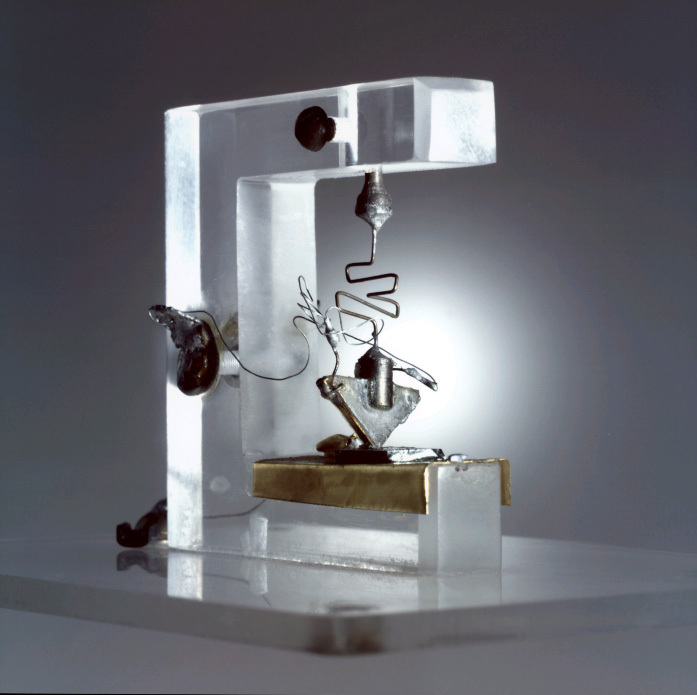
\includegraphics[trim={15mm 10mm 15mm 15mm}, clip]{figs/First_point_contact_transistor_1947.jpg}}};
		\node[block] (C2) at ($(C1.east) + (2.2cm,0)$) {\resizebox{!}{3.2cm}{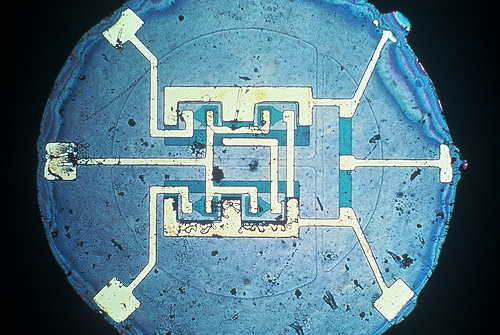
\includegraphics[trim={3mm 0 3mm 0}, clip]{figs/first_ic_1961.jpg}}};
		\node[block] (C3) at ($(C2.east) + (2.5cm,0)$)  {\resizebox{!}{3.2cm}{\includegraphics{figs/modern_i7.jpg}}};
		\node[below=0.2cm of C1, text width=4cm, align=center] (cap1) {First point contact transistor (1947)};
		\node[below=0.2cm of C2, text width=4.2cm, align=center] (cap2) {First integrated circuit (1961)};
		\node[below=0.2cm of C3, text width=4cm, align=center] (cap3) {Modern processor (200X)};	
	\end{tikzpicture}
}	
\end{frame}

%
\begin{frame}{Why learn DSP?}

\begin{itemize}
	\item Present in essentially all fields of modern EE
    \item Countless applications
    \vspace{0.25cm}
    
	\begin{center}
		\resizebox{\linewidth}{!}{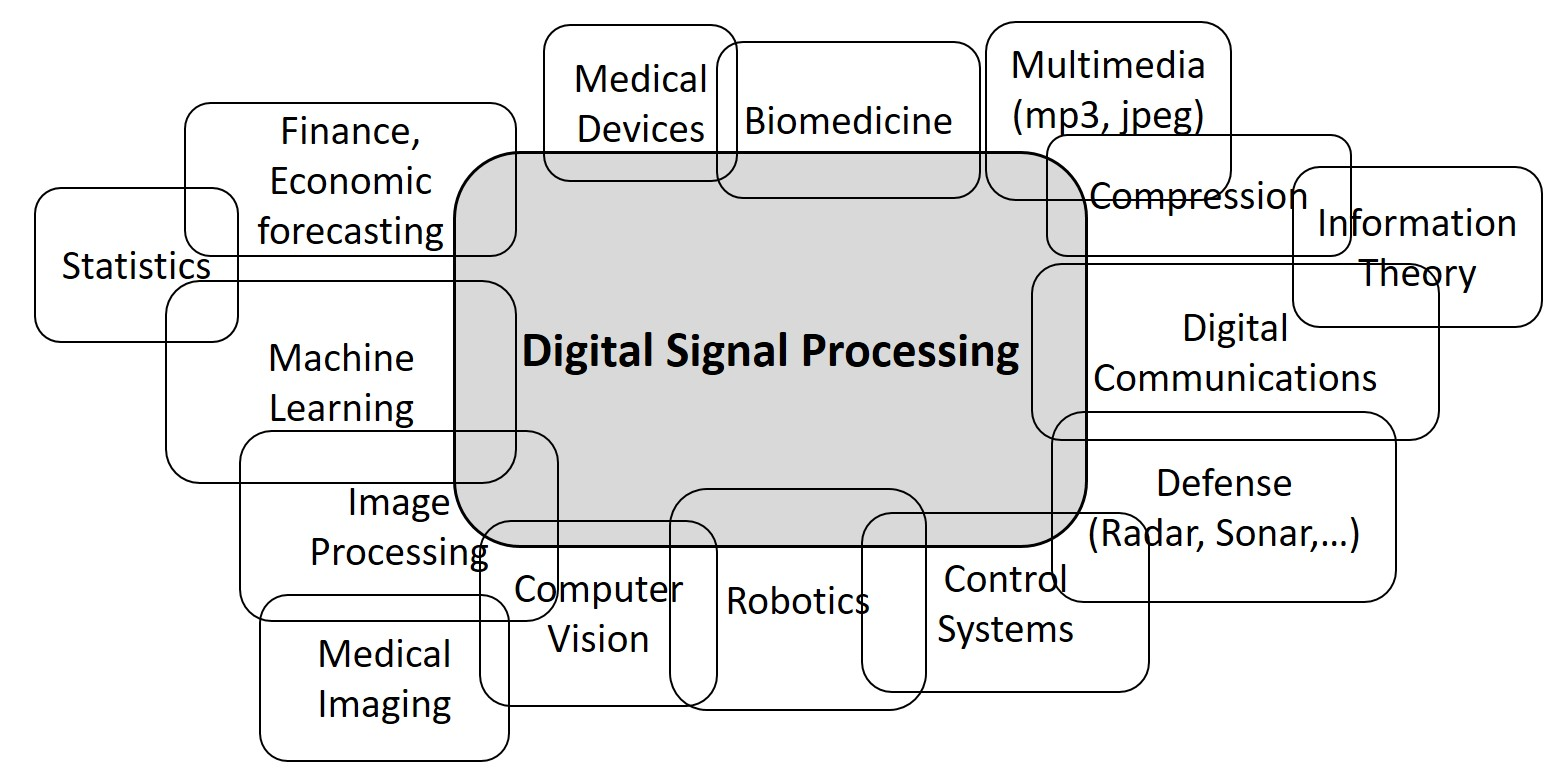
\includegraphics{figs/ee264_and_related_areas.jpg}}
	\end{center}
\end{itemize}

\end{frame}

%
\begin{frame}{Example: digital communication}

\begin{block}{Problem:}
\begin{figure}
	\centering
	\resizebox{0.7\linewidth}{!}{\def\layersep{1.5cm}
\def\outsep{0.7cm}
\def\dy{1.25}

\begin{tikzpicture}[draw=black!50, node distance=\layersep, font=\sffamily]
    \tikzstyle{node}=[circle,fill=black,minimum size=2pt,inner sep=0pt]
    \tikzstyle{block}=[draw=black,rectangle,fill=none,minimum size=1.5cm, inner sep=0pt]
    \tikzstyle{annot} = []

	\node[node] (xc) at (0, -\dy cm) {};
	
    \onslide<1|handout:1>{\node[block, text width = 2cm, align= center] (CH) at (2*\layersep, -\dy cm) {Channel};}
    
    \onslide<2-|handout:2->{\node[block, text width = 2cm, align= center] (CH) at (2*\layersep, -\dy cm) {Bad Channel};}
    
	\coordinate (yc) at (4*\layersep, -\dy cm) {};
		
    \path[->, >=stealth, shorten >= 0pt] (xc) edge (CH);
    \path[->, >=stealth, shorten >= 0pt] (CH) edge (yc);
    
    \node[block, draw=none, above = 0.5mm of xc, scale=0.5] (tx_signal) {\resizebox{!}{!}{\begin{tikzpicture}
\begin{axis}[
width=4.52in,
height=3.56in,
scale only axis,
separate axis lines,
every outer x axis line/.append style={white!15!black},
every x tick label/.append style={font=\color{white!15!black}},
xmin=0.00,
xmax=70.00,
ymin=0.00,
ymax=1.00,
xlabel={},
ylabel={},
xmajorgrids,
ymajorgrids,
every outer y axis line/.append style={white!15!black},
every y tick label/.append style={font=\color{white!15!black}},
legend style={draw=white!15!black,fill=white,legend cell align=left}]
\definecolor{matlabColor1}{rgb}{0.000000,0.447000,0.741000}
\addplot [color=matlabColor1, solid, line width=1.5pt, forget plot]
table[row sep=crcr]{
	1 0 \\
	2 0 \\
	3 0 \\
	4 0 \\
	5 0 \\
	6 0 \\
	7 0 \\
	8 0 \\
	9 0 \\
	10 0 \\
	11 0 \\
	12 1 \\
	13 1 \\
	14 1 \\
	15 1 \\
	16 1 \\
	17 1 \\
	18 1 \\
	19 1 \\
	20 1 \\
	21 1 \\
	22 1 \\
	23 0 \\
	24 0 \\
	25 0 \\
	26 0 \\
	27 0 \\
	28 0 \\
	29 0 \\
	30 0 \\
	31 0 \\
	32 0 \\
	33 0 \\
	34 1 \\
	35 1 \\
	36 1 \\
	37 1 \\
	38 1 \\
	39 1 \\
	40 1 \\
	41 1 \\
	42 1 \\
	43 1 \\
	44 1 \\
	45 1 \\
	46 1 \\
	47 1 \\
	48 1 \\
	49 1 \\
	50 1 \\
	51 1 \\
	52 1 \\
	53 1 \\
	54 1 \\
	55 1 \\
	56 0 \\
	57 0 \\
	58 0 \\
	59 0 \\
	60 0 \\
	61 0 \\
	62 0 \\
	63 0 \\
	64 0 \\
	65 0 \\
	66 0 \\
};

\end{axis}
\end{tikzpicture}}};
    \onslide<1|handout:1>\node[block, draw=none, above = 0.5mm of yc, scale=0.5] (tx_signal) {\resizebox{!}{!}{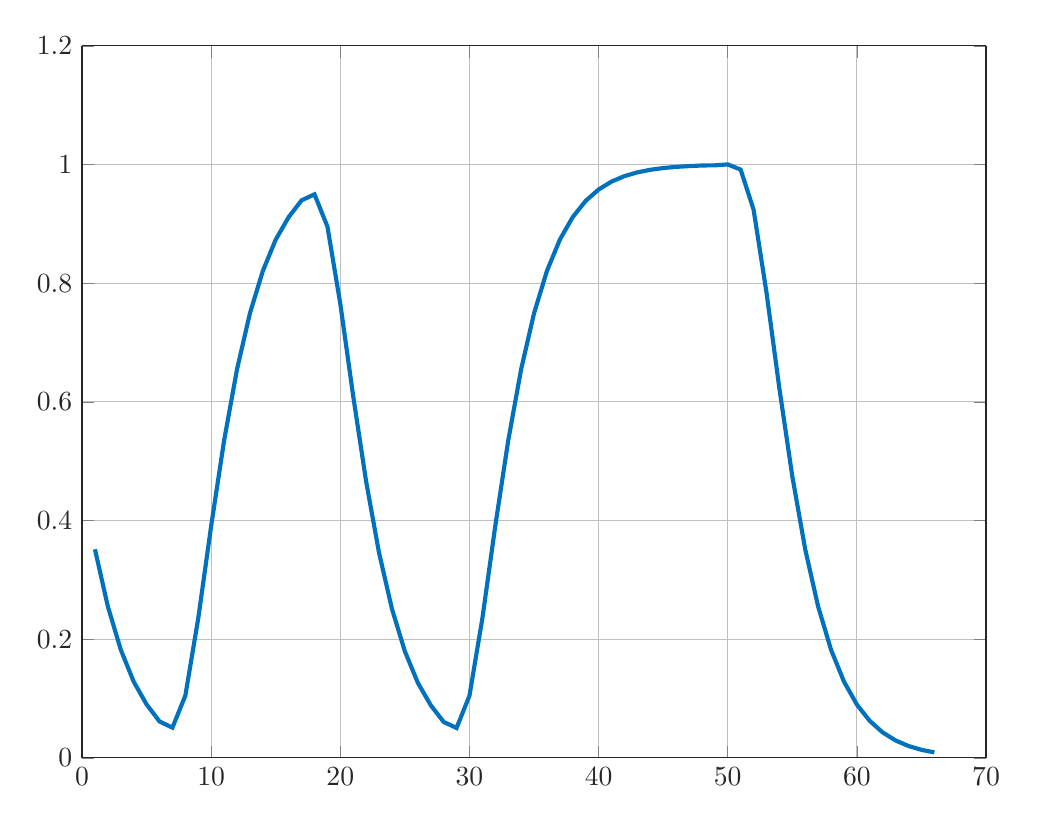
\begin{tikzpicture}
\begin{axis}[
width=4.52in,
height=3.56in,
scale only axis,
separate axis lines,
every outer x axis line/.append style={white!15!black},
every x tick label/.append style={font=\color{white!15!black}},
xmin=0.00,
xmax=70.00,
ymin=0.00,
ymax=1.20,
xlabel={},
ylabel={},
xmajorgrids,
ymajorgrids,
every outer y axis line/.append style={white!15!black},
every y tick label/.append style={font=\color{white!15!black}},
legend style={draw=white!15!black,fill=white,legend cell align=left}]
\definecolor{matlabColor1}{rgb}{0.000000,0.447000,0.741000}
\addplot [color=matlabColor1, solid, line width=1.5pt, forget plot]
table[row sep=crcr]{
	1 0.35141 \\
	2 0.25498 \\
	3 0.18215 \\
	4 0.12838 \\
	5 0.089941 \\
	6 0.06127 \\
	7 0.050858 \\
	8 0.10489 \\
	9 0.23518 \\
	10 0.39096 \\
	11 0.5346 \\
	12 0.65469 \\
	13 0.7491 \\
	14 0.82058 \\
	15 0.87344 \\
	16 0.91127 \\
	17 0.93953 \\
	18 0.94968 \\
	19 0.89546 \\
	20 0.76505 \\
	21 0.60919 \\
	22 0.4655 \\
	23 0.34537 \\
	24 0.25094 \\
	25 0.17945 \\
	26 0.12658 \\
	27 0.08874 \\
	28 0.060478 \\
	29 0.050327 \\
	30 0.10455 \\
	31 0.23495 \\
	32 0.39082 \\
	33 0.53449 \\
	34 0.65464 \\
	35 0.74903 \\
	36 0.8206 \\
	37 0.87333 \\
	38 0.91149 \\
	39 0.93866 \\
	40 0.95781 \\
	41 0.97113 \\
	42 0.98037 \\
	43 0.98669 \\
	44 0.99104 \\
	45 0.99395 \\
	46 0.99598 \\
	47 0.99725 \\
	48 0.99829 \\
	49 0.99857 \\
	50 1.0001 \\
	51 0.99134 \\
	52 0.92397 \\
	53 0.78446 \\
	54 0.62233 \\
	55 0.47438 \\
	56 0.35133 \\
	57 0.25497 \\
	58 0.18208 \\
	59 0.12846 \\
	60 0.089692 \\
	61 0.062127 \\
	62 0.042717 \\
	63 0.029214 \\
	64 0.01986 \\
	65 0.01346 \\
	66 0.0090624 \\
};

\end{axis}
\end{tikzpicture}}};
    \onslide<2-|handout:2->\node[block, draw=none, above = 0.5mm of yc, scale=0.5] (tx_signal) {\resizebox{!}{!}{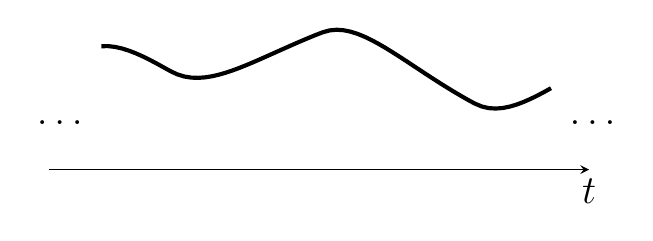
\begin{tikzpicture}
\begin{axis}[
axis lines*=middle,
enlargelimits = true,
hide y axis,
axis line style={->,>=stealth},
xmin=0.00,
xmax= 65.00,
ymin=0.00,
ymax=2.00,
clip=false,
xlabel={\Large $t$},
ylabel={},
xtick=\empty,
ytick=\empty,
every axis x label/.style={
	at={(ticklabel* cs:1)},
	anchor=north,
},
]
\node at (axis cs: 72, 0.25) {\Large$\ldots$};
\node at (axis cs: -5, 0.25) {\Large$\ldots$};
\addplot [color=black, solid, line width=1.5pt, forget plot]
table[row sep=crcr]{
	1 0.6606 \\
	2 0.66119 \\
	3 0.65685 \\
	4 0.64848 \\
	5 0.63679 \\
	6 0.6224 \\
	7 0.60585 \\
	8 0.58762 \\
	9 0.56813 \\
	10 0.54763 \\
	11 0.52712 \\
	12 0.50985 \\
	13 0.49845 \\
	14 0.49258 \\
	15 0.49132 \\
	16 0.49395 \\
	17 0.4998 \\
	18 0.50832 \\
	19 0.519 \\
	20 0.53142 \\
	21 0.5452 \\
	22 0.56002 \\
	23 0.57562 \\
	24 0.59174 \\
	25 0.60818 \\
	26 0.62478 \\
	27 0.64139 \\
	28 0.65789 \\
	29 0.67417 \\
	30 0.69016 \\
	31 0.70577 \\
	32 0.72103 \\
	33 0.73522 \\
	34 0.7453 \\
	35 0.74884 \\
	36 0.74634 \\
	37 0.73887 \\
	38 0.72727 \\
	39 0.7123 \\
	40 0.69462 \\
	41 0.67481 \\
	42 0.65334 \\
	43 0.63065 \\
	44 0.60709 \\
	45 0.58298 \\
	46 0.55858 \\
	47 0.53412 \\
	48 0.50978 \\
	49 0.48573 \\
	50 0.46207 \\
	51 0.43893 \\
	52 0.41638 \\
	53 0.39451 \\
	54 0.37328 \\
	55 0.35341 \\
	56 0.33794 \\
	57 0.32928 \\
	58 0.32694 \\
	59 0.32982 \\
	60 0.33708 \\
	61 0.34795 \\
	62 0.36176 \\
	63 0.37793 \\
	64 0.39597 \\
	65 0.41544 \\
	66 0.43596 \\
};

\end{axis}
\end{tikzpicture}}};

\end{tikzpicture}}
\end{figure}
\end{block}

\onslide<3-|handout:2->{\begin{block}{Solution:}
	\begin{figure}
		\centering
		\resizebox{\linewidth}{!}{\def\layersep{5.5cm}
\def\outsep{0.7cm}
\def\dy{1.25}

\begin{tikzpicture}[draw=black!50, node distance=\layersep, font=\sffamily]
    \tikzstyle{node}=[circle,fill=black,minimum size=2pt,inner sep=0pt]
    \tikzstyle{block}=[draw=black,rectangle,fill=none,minimum size=1.5cm, inner sep=0pt]
    \tikzstyle{annot} = []

	\node[node] (xc) at (0, -\dy cm) {};
	
    \node[block, text width = 2cm, align= center, right=2cm of xc] (CH) {Channel};
    \node[block, text width = 2cm, align= center, right of=CH] (ADC)  {Analog-to-Digital Conveter};
    \node[block, text width = 2cm, align= center, right of=ADC] (EQ)  {Equalizer};
	\coordinate[right=2cm of EQ] (yc) {};
		
    \path[->, >=stealth, shorten >= 0pt] (xc) edge (CH);
    \path[->, >=stealth, shorten >= 0pt] (CH) edge (ADC);
    \path[->, >=stealth, shorten >= 0pt] (ADC) edge (EQ);
    \path[->, >=stealth, shorten >= 0pt] (EQ) edge (yc);
    
    \node[block, draw=none, above = 0.5mm of xc, scale=0.45] (tx_signal) {\resizebox{!}{!}{\begin{tikzpicture}
\begin{axis}[
width=4.52in,
height=3.56in,
scale only axis,
separate axis lines,
every outer x axis line/.append style={white!15!black},
every x tick label/.append style={font=\color{white!15!black}},
xmin=0.00,
xmax=70.00,
ymin=0.00,
ymax=1.00,
xlabel={},
ylabel={},
xmajorgrids,
ymajorgrids,
every outer y axis line/.append style={white!15!black},
every y tick label/.append style={font=\color{white!15!black}},
legend style={draw=white!15!black,fill=white,legend cell align=left}]
\definecolor{matlabColor1}{rgb}{0.000000,0.447000,0.741000}
\addplot [color=matlabColor1, solid, line width=1.5pt, forget plot]
table[row sep=crcr]{
	1 0 \\
	2 0 \\
	3 0 \\
	4 0 \\
	5 0 \\
	6 0 \\
	7 0 \\
	8 0 \\
	9 0 \\
	10 0 \\
	11 0 \\
	12 1 \\
	13 1 \\
	14 1 \\
	15 1 \\
	16 1 \\
	17 1 \\
	18 1 \\
	19 1 \\
	20 1 \\
	21 1 \\
	22 1 \\
	23 0 \\
	24 0 \\
	25 0 \\
	26 0 \\
	27 0 \\
	28 0 \\
	29 0 \\
	30 0 \\
	31 0 \\
	32 0 \\
	33 0 \\
	34 1 \\
	35 1 \\
	36 1 \\
	37 1 \\
	38 1 \\
	39 1 \\
	40 1 \\
	41 1 \\
	42 1 \\
	43 1 \\
	44 1 \\
	45 1 \\
	46 1 \\
	47 1 \\
	48 1 \\
	49 1 \\
	50 1 \\
	51 1 \\
	52 1 \\
	53 1 \\
	54 1 \\
	55 1 \\
	56 0 \\
	57 0 \\
	58 0 \\
	59 0 \\
	60 0 \\
	61 0 \\
	62 0 \\
	63 0 \\
	64 0 \\
	65 0 \\
	66 0 \\
};

\end{axis}
\end{tikzpicture}}};
    \node[block, draw=none, scale=0.45] at ($(CH.east)!0.5!(ADC.west) + (0, 1cm)$) (rx_signal) {\resizebox{!}{!}{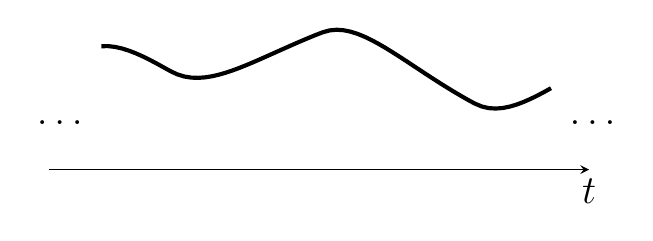
\begin{tikzpicture}
\begin{axis}[
axis lines*=middle,
enlargelimits = true,
hide y axis,
axis line style={->,>=stealth},
xmin=0.00,
xmax= 65.00,
ymin=0.00,
ymax=2.00,
clip=false,
xlabel={\Large $t$},
ylabel={},
xtick=\empty,
ytick=\empty,
every axis x label/.style={
	at={(ticklabel* cs:1)},
	anchor=north,
},
]
\node at (axis cs: 72, 0.25) {\Large$\ldots$};
\node at (axis cs: -5, 0.25) {\Large$\ldots$};
\addplot [color=black, solid, line width=1.5pt, forget plot]
table[row sep=crcr]{
	1 0.6606 \\
	2 0.66119 \\
	3 0.65685 \\
	4 0.64848 \\
	5 0.63679 \\
	6 0.6224 \\
	7 0.60585 \\
	8 0.58762 \\
	9 0.56813 \\
	10 0.54763 \\
	11 0.52712 \\
	12 0.50985 \\
	13 0.49845 \\
	14 0.49258 \\
	15 0.49132 \\
	16 0.49395 \\
	17 0.4998 \\
	18 0.50832 \\
	19 0.519 \\
	20 0.53142 \\
	21 0.5452 \\
	22 0.56002 \\
	23 0.57562 \\
	24 0.59174 \\
	25 0.60818 \\
	26 0.62478 \\
	27 0.64139 \\
	28 0.65789 \\
	29 0.67417 \\
	30 0.69016 \\
	31 0.70577 \\
	32 0.72103 \\
	33 0.73522 \\
	34 0.7453 \\
	35 0.74884 \\
	36 0.74634 \\
	37 0.73887 \\
	38 0.72727 \\
	39 0.7123 \\
	40 0.69462 \\
	41 0.67481 \\
	42 0.65334 \\
	43 0.63065 \\
	44 0.60709 \\
	45 0.58298 \\
	46 0.55858 \\
	47 0.53412 \\
	48 0.50978 \\
	49 0.48573 \\
	50 0.46207 \\
	51 0.43893 \\
	52 0.41638 \\
	53 0.39451 \\
	54 0.37328 \\
	55 0.35341 \\
	56 0.33794 \\
	57 0.32928 \\
	58 0.32694 \\
	59 0.32982 \\
	60 0.33708 \\
	61 0.34795 \\
	62 0.36176 \\
	63 0.37793 \\
	64 0.39597 \\
	65 0.41544 \\
	66 0.43596 \\
};

\end{axis}
\end{tikzpicture}}};
	\node[block, draw=none, scale=0.45] at ($(ADC.east)!0.5!(EQ.west) + (0, 1cm)$) (rx_signal_sampled) {\resizebox{!}{!}{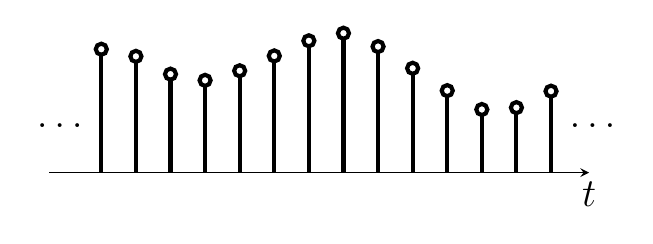
\begin{tikzpicture}
\begin{axis}[
axis lines*=middle,
enlargelimits = true,
clip=false,
hide y axis,
axis line style={->,>=stealth},
xmin=0.00,
xmax= 65.00,
ymin=0.00,
ymax=2.00,
xlabel={\Large $t$},
ylabel={},
xtick=\empty,
ytick=\empty,
every axis x label/.style={
	at={(ticklabel* cs:1)},
	anchor=north,
},
]
\node at (axis cs: 72, 0.25) {\Large$\ldots$};
\node at (axis cs: -5, 0.25) {\Large$\ldots$};
\addplot [ycomb, color=black, solid, mark=*, mark options={fill=white}, line width=1.5pt, forget plot, each nth point={5}]
table[row sep=crcr]{
	1 0.6606 \\
	2 0.66119 \\
	3 0.65685 \\
	4 0.64848 \\
	5 0.63679 \\
	6 0.6224 \\
	7 0.60585 \\
	8 0.58762 \\
	9 0.56813 \\
	10 0.54763 \\
	11 0.52712 \\
	12 0.50985 \\
	13 0.49845 \\
	14 0.49258 \\
	15 0.49132 \\
	16 0.49395 \\
	17 0.4998 \\
	18 0.50832 \\
	19 0.519 \\
	20 0.53142 \\
	21 0.5452 \\
	22 0.56002 \\
	23 0.57562 \\
	24 0.59174 \\
	25 0.60818 \\
	26 0.62478 \\
	27 0.64139 \\
	28 0.65789 \\
	29 0.67417 \\
	30 0.69016 \\
	31 0.70577 \\
	32 0.72103 \\
	33 0.73522 \\
	34 0.7453 \\
	35 0.74884 \\
	36 0.74634 \\
	37 0.73887 \\
	38 0.72727 \\
	39 0.7123 \\
	40 0.69462 \\
	41 0.67481 \\
	42 0.65334 \\
	43 0.63065 \\
	44 0.60709 \\
	45 0.58298 \\
	46 0.55858 \\
	47 0.53412 \\
	48 0.50978 \\
	49 0.48573 \\
	50 0.46207 \\
	51 0.43893 \\
	52 0.41638 \\
	53 0.39451 \\
	54 0.37328 \\
	55 0.35341 \\
	56 0.33794 \\
	57 0.32928 \\
	58 0.32694 \\
	59 0.32982 \\
	60 0.33708 \\
	61 0.34795 \\
	62 0.36176 \\
	63 0.37793 \\
	64 0.39597 \\
	65 0.41544 \\
	66 0.43596 \\
};

\end{axis}
\end{tikzpicture}}};	\node[block, draw=none, above = 0.5mm of yc]  (detected) {010110};

\end{tikzpicture}}
		\label{fig:channel_eq}
	\end{figure}
\end{block}

More about filter design on lecture 9
}

\end{frame}


%
\begin{frame}{Example: speech recognition}
\centering
\vspace{1cm}
\begin{tikzpicture}[draw=black!50, node distance=1cm]
	\tikzstyle{block}=[draw=none,rectangle,fill=none,minimum size=1.5cm, inner sep=0pt]
	\node[block] (C1) {\resizebox{0.8\textwidth}{!}{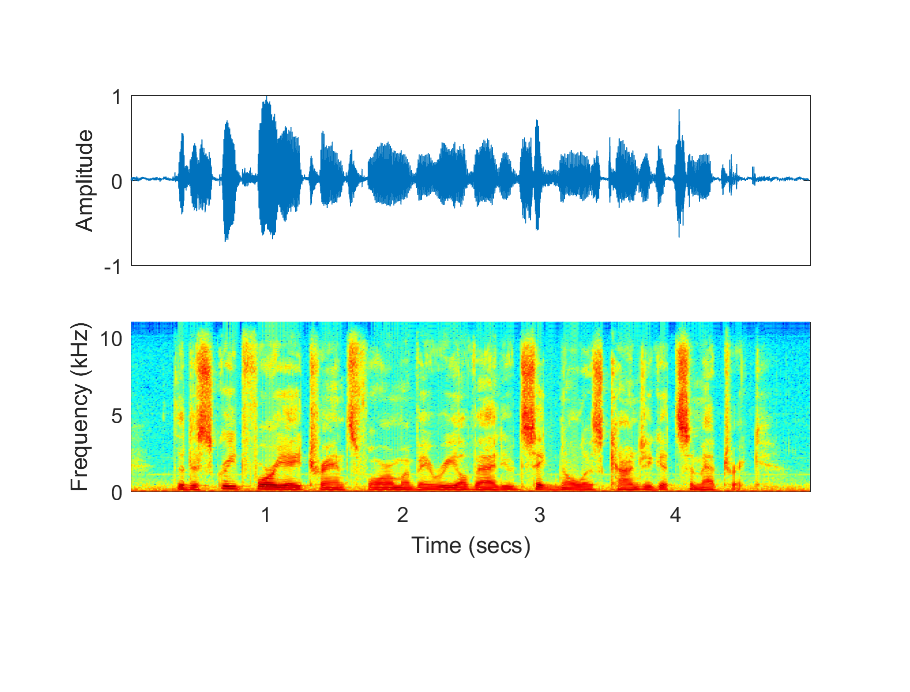
\includegraphics[trim={2cm 2cm 2cm 2cm}]{figs/speech_spectogram.eps}}};
	
	\node (the) at (-3.6, 1.2) {\tiny The};
	\node (discrete) at ($(the.east) + (0.43,0)$) {\tiny discrete};
	\node (fourier) at ($(discrete.east) + (0.2,0)$) {\tiny Fourier};
	\node (transform) at ($(fourier.east) + (0.6,0)$) {\tiny transform of a};
	\node[align=left] (real) at ($(transform.east) + (0.4,0)$) {\tiny r~e~a~l};
	\node[align=left] (valued) at ($(real.east) + (0.3,0)$) {\tiny valued};
	\node[align=left] (signal) at ($(valued.east) + (0.59,0)$) {\tiny sig~~~~~n~a~l is};
	\node[align=left] (conjugate) at ($(signal.east) + (0.37,0)$) {\tiny conjugate};
	\node[align=left] (symmetric) at ($(conjugate.east) + (0.4,0)$) {\tiny symmetric};
	%\draw 
\end{tikzpicture}

\end{frame}

%
\begin{frame}{Example: speech recognition}

\centering
\resizebox{0.8\linewidth}{!}{\def\layersep{3cm}
\def\outsep{0.7cm}
\def\dy{1.5}

\begin{tikzpicture}[->, >=stealth, shorten >= 0pt, draw=black!50, node distance=\layersep, font=\sffamily]
    \tikzstyle{node}=[circle,fill=black,minimum size=2pt,inner sep=0pt]
    \tikzstyle{block}=[draw=black,rectangle,fill=none,minimum size=1cm, inner sep=0pt]
    \tikzstyle{annot} = []

	\node[node] (xc) at (0, 0 cm) {};
    \node[block, minimum size=2cm, text width=2cm, align=center] (RNN) at (1*\layersep, 0 cm) {Recurrent Neural Network};
	\node[block, text width=2cm, align=center] (O1) at (2*\layersep, \dy cm) {Probability of begin `A'};
	\node[block, text width=2cm, align=center] (O2) at (2*\layersep, 0 cm) {Probability of begin `B'};
	\node[block, text width=2cm, align=center] (O3) at (2*\layersep, -\dy cm) {Probability of begin `C'};
	\node (vdots) at (2*\layersep, -1.5*\dy cm) {\Large $\vdots$};
			
			
    \path (xc) edge (RNN);
    \path (RNN.east) edge (O1.west);
    \path (RNN.east) edge (O2.west);
    \path (RNN.east) edge (O3.west);    
    \draw (RNN) to[loop above]  (RNN);
    
    \node[left = 0mm of xc] (spectrogram) {\resizebox{!}{0.7\textheight}{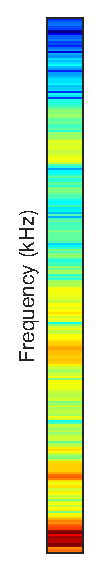
\includegraphics{figs/speech_spectogram_strip.eps}}};
    \node[below = 1mm of spectrogram, text width=2cm, align=center] {Slice of the spectrogram};
    
\end{tikzpicture}}

\end{frame}

%
\begin{frame}{Example: speech recognition}

Spectrogram of the same speech signal, now recorded with sampling rate of 44.1 kHz
\vspace{0.5cm}

\begin{center}
\resizebox{0.7\textwidth}{!}{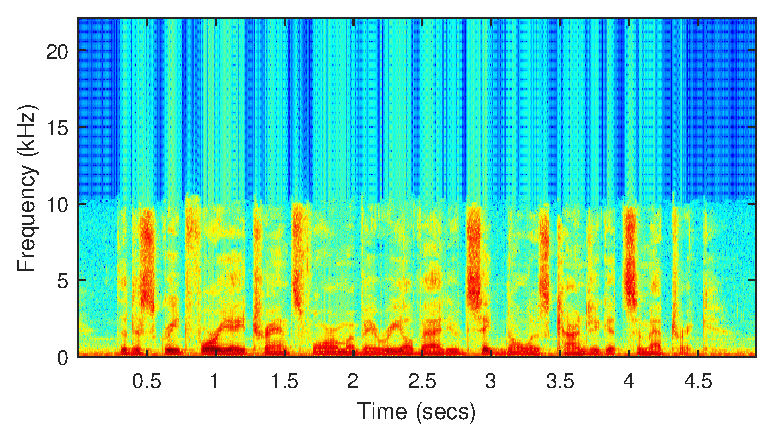
\includegraphics{figs/speech_spectogram_44k.eps}}
\end{center}

More on spectrograms and short-time Fourier transform on lecture 12.

\end{frame}


%%%%%%%%%%%%%%%%%%%%%%%%%
\section{Administrative}

%
\begin{frame}{Administrative: tentative schedule and class topics}

\centering
\resizebox{\linewidth}{!}{\begin{tabular}{c|c|l|c|c}
	\hline
	Date & Lecture	& Lecture Topic	& Reading\footnotemark & Assigned \\
	\hline
	25-Jun	& 1 &	Introduction and review			& Chaps. 2, 3	& \\
	27-Jun	& 2 &	Discrete-time random signals	& 2.10, App. A & HW1\\
	29-Jun 	& 3 & 	Properties of LTI systems 		& 5.1--5.7 	&  \\
	\hline
	2-Jul	& 	& 	\textbf{No lecture (make-up lecture on Jun 29)}	&  & \\
	4-Jul	&  & 	Independence Day, no classes  	&		& HW2 \\
	\hline
	9-Jul	& 4 & 	Sampling and reconstruction  	& 4.1--4.4 	& \\
	11-Jul	& 5	& 	Changing the sampling rate by digital filtering	& 4.6--4.9 		& HW3 \\
	\hline
	16-Jul	& 6	& 	Digital filter structures				& 6.1--6.6 & \\
	18-Jul	& 7	& 	Quantization and finite-precision arithmetic &	6.7--6.10	& \\
	20-Jul	& 	& 	Midterm review session (11:30 AM--11:20 PM in \href{https://campus-map.stanford.edu/?srch=Gates+Computer+Science}{Gates B3})  & & \\
	\hline
	23-Jul	& 	& 	In-class midterm exam (Lecs. 1--7, HWs 1--3) & & \\
	25-Jul	& 8	& 	Filter design & Chap. 7	& HW4 \\
	\hline
	30-Jul	& 9 & 	Adaptive signal processing & & \\
	1-Aug	& 10 & 	The discrete Fourier transform (DFT) & 8.1--8.7, 9.1--9.3	& HW5 \\
	\hline
	6-Aug	& 11 & 	Time-dependent Fourier transform	& 10.1--10.4 & \\
	8-Aug	& 12 & 	Power spectrum density estimation & 10.5, 10.6 & HW6 \\
	\hline
	13-Aug	& 13 & 	Parametric signal modeling 	& 11.1--11.6	& \\
	15-Aug 	& 14 & 	Review and conclusions &  & 	\\
	TBD	& 	 & 	24-hour-take-home final exam & \\
	\hline
\end{tabular}}
\footnotetext[1]{Reading assignments in ``Discrete-Time Signal Processing'', Oppenheim and Schafer, 3rd edition}

\end{frame}

%
\begin{frame}{Administrative: resources}
\begin{block}{Textbook}
\begin{columns}[t]
	\begin{column}{0.8\textwidth}
		\begin{itemize}
			\item ``Discrete-Time Signal Processing'', Oppenheim and Schafer, 3rd edition, 2010.
			\item Available on 4-hour reserve at the \href{https://campus-map.stanford.edu/?id=04-080&lat=37.42787956&lng=-122.17429865&zoom=17&srch=engineeri}{Engineering Library (Terman)}
		\end{itemize}
	\end{column}
	\begin{column}{0.25\textwidth}  %%<--- here
		\vspace{-1cm}
		\begin{center}
			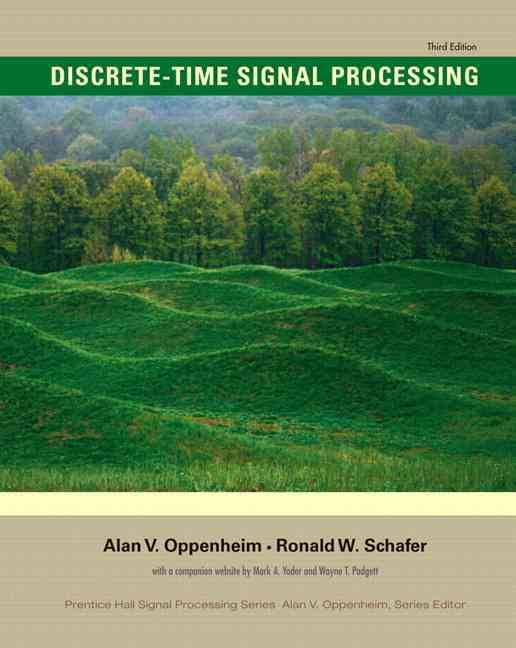
\includegraphics[width=\textwidth]{figs/book_cover.jpg}
		\end{center}
	\end{column}
\end{columns}
\end{block}
\vspace{-0.5cm}
\begin{block}{Lecture notes}
	\begin{itemize}
		\item Lecture notes will cover all the material, but further reading of the textbook is encouraged.
	\end{itemize}
\end{block}

\begin{block}{Canvas: \href{https://canvas.stanford.edu}{canvas.stanford.edu}}
	\begin{itemize}
		\item Lecture notes, homework assignments and solutions, Matlab code, discussion
		\item Submit homework on Canvas
	\end{itemize}
\end{block}

\end{frame}

%
\begin{frame}{Administrative: homework assignments}

\begin{itemize}
	\item Assignments will typically be released on Thursday and will be due on the following Thursday at 11:59pm
	\item Submit a single .pdf file with your solutions online on Canvas
	\item Homework assignments include analytical derivations and Matlab simulations
	\item Discussion among students is encouraged, but individual solutions must be submitted
	\item Late homeworks will be not accepted
\end{itemize}

\end{frame}

%
\begin{frame}{Administrative: exams}
	
\begin{block}{Midterm}
	\begin{itemize} 
	\item In-class midterm on August, 1st. 
	\item There will be a midterm review session on Friday, July 28. Time and location TBD
	\item Midterm covers lectures 1 to 8 (homeworks 1 to 4)
	\item Midterm is open book and open notes
	\end{itemize}
\end{block}

\begin{block}{Final}
	\begin{itemize} 
	\item Final exam will be a 24-hour take home exam. Dates TBD
	\item The final exam should take just a few hours
	\item The review session for the final will be on the last lecture
	\end{itemize}
\end{block}

\end{frame}

%
\begin{frame}{Administrative: grading}
	
	\begin{itemize}
		\item Homework assignments: $30\%$
		\item Midterm: $30\%$
		\item Final: $40\%$
	\end{itemize}
	
\end{frame}

%
\begin{frame}{Administrative: enrollment}
	
\begin{itemize}
	\item Please \textbf{enroll for 3 units}. EE 264 is only offered for 4 units during the Winter quarter.
	\item The deadline to adjust units is July 7.
\end{itemize}
	
\end{frame}

%%%%%%%%%%%%%%%%%%%%%%%%%
\section{Review}

%
\begin{frame}{Review}
	\begin{itemize}
		\item Discrete-time signals and systems
		\item Discrete-time Fourier transform (DTFT)
		\item The $z$-transform
		\item Difference equations
	\end{itemize}
\end{frame}

%
\begin{frame}{Digital processing of analog signals}
\vspace{-0.5cm}
\begin{figure}[t!]
	\centering
	\resizebox{\linewidth}{!}{\def\layersep{1.5cm}
\def\outsep{0.7cm}
\def\dy{1.25}

\begin{tikzpicture}[->, >=stealth, shorten >= 0pt, draw=black!50, node distance=\layersep, font=\sffamily]
    \tikzstyle{node}=[circle,fill=black,minimum size=2pt,inner sep=0pt]
    \tikzstyle{block}=[draw=black,rectangle,fill=none,minimum size=1.5cm, inner sep=0pt]
    \tikzstyle{annot} = []

	\node[node] (xc) at (0, -\dy cm) {};
    \node[block] (ADC) at (1*\layersep, -\dy cm) {ADC};
    \node[block, text width = 2.5cm, align= center] (DSP) at (3*\layersep, -\dy cm) {Digital Signal Processor};
    \node[block] (DAC) at (5*\layersep, -\dy cm) {DAC};
	\coordinate (yc) at (6*\layersep, -\dy cm) {};
	
	\coordinate (mid1) at ($(ADC.east)!0.5!(DSP.west)$) {};
	\coordinate (mid2) at ($(DSP.east)!0.5!(DAC.west)$) {};
		
    \path (xc) edge (ADC);
    \path (ADC) edge (DSP);
    \path (DSP) edge (DAC);
    \path (DAC) edge (yc);
    
    \node[above = 0.5mm of mid1] {$x[n]$};
    \node[above = 0.5mm of mid2] {$y[n]$};
    \node[left = 0mm of xc, text width = 1cm, align=center] {$x_c(t)$};
    \node[right = 0mm of yc, text width = 1cm, align=center] {$y_c(t)$}; 
    

\end{tikzpicture}}
	\label{fig:adc-dsp-dac}
\end{figure}
\vspace{-0.5cm}
\begin{block}{Analog-to-digital converter (ADC)}
	\begin{itemize}
		\item Performs filtering, sampling, and quantization
		\item Sampling rate may be of tens of kHz (audio processing), or it may be of tens of GHz (optical communications)
	\end{itemize}
\end{block}
\vspace{-0.3cm}
\begin{block}{Digital signal processor}
	\begin{itemize} \itemsep 0pt
		\item Performs some operation e.g., filtering, FFT, etc
		\item May be implemented on PCs with 64-bit floating-point precision, or on ASICs with limited arithmetic precision (e.g., 6 bits).
	\end{itemize}
\end{block}
\vspace{-0.3cm}
\begin{block}{Digital-to-analog converter (DAC)}
	\begin{itemize}
		\item Performs quantization and reconstruction (filtering)
		\item Sampling rate could be similar to ADC
	\end{itemize}
\end{block}

\end{frame}

\subsection{The Discrete-Time Signals and Systems}
%
\begin{frame}{Discrete-time signals}

Discrete-time signals (or simply \textit{sequences}) may be inherently discrete or they may be obtained by sampling a continuous-time signal. More about sampling on lecture 3.

\begin{figure}[t!]
	\centering
	\resizebox{0.5\linewidth}{!}{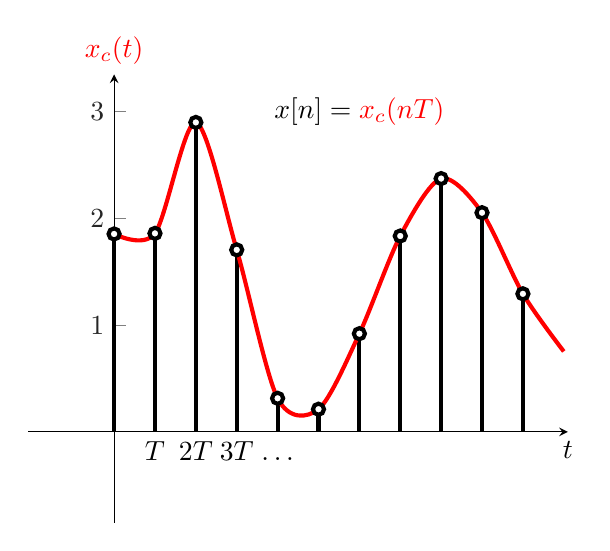
\begin{tikzpicture} 
\begin{axis}[
axis lines*=middle,
enlargelimits = true,
xmin=-1,
xmax=10,
ymin=-0.5,
ymax=3,
axis line style={->,>=stealth},
xlabel={$t$},
ylabel={$\textcolor{red}{x_c(t)}$},
%yticklabel style = {yshift=0.2cm},
every axis x label/.style={
    at={(ticklabel* cs:1)},
    anchor=north,
},
every axis y label/.style={
    at={(ticklabel* cs:1)},
    anchor=south,
},
xtick={0, 1, ..., 3},
%ytick={1},
%xtick={-3.14, -1, 1, 3.14},
xticklabels={0, $T$, $2T$, $3T$},
%xmajorgrids,
%ymajorgrids,
every outer y axis line/.append style={white!15!black},
every y tick label/.append style={font=\color{white!15!black}},
legend style={draw=white!15!black,fill=white,legend cell align=left}]

\pgfmathsetseed{103}
\addplot[ycomb, mark=*, line width=2pt, domain=0:10, samples=11, line width=1.5, mark options={scale=1,fill=white}] {sin(deg(x)) + 0.5*rand + 1.5};
\pgfmathsetseed{103}
\addplot[red, smooth, line width=2pt, domain=0:11, samples=12, line width=1.5] {sin(deg(x)) + 0.5*rand + 1.5};
\node (dots) at (axis cs: 4, -0.25) {$\ldots$};
\node at (axis cs: 6, 3) {$x[n] = \textcolor{red}{x_c(nT)}$};
\end{axis}
\end{tikzpicture}
}
	\label{fig:ct_signal_sampled}
\end{figure}

$x[n]$ is only defined for $n\in\mathbb{Z}$
\end{frame}

%
\begin{frame}{Basic sequences}
	\begin{columns}[t]
		\begin{column}{0.5\linewidth}
			\textbf{Unit impulse:} 
			
			\begin{equation*}
				\delta[n] = \begin{cases}
				1, & n = 0 \\
				0, & \text{otherwise}
				\end{cases}
			\end{equation*}
		\end{column}		
		
		\begin{column}{0.5\linewidth}
			\textbf{Unit step:} 
			\begin{equation*}
				u[n] = \begin{cases}
				1, & n \geq 0 \\
				0, & \text{otherwise}
				\end{cases}
			\end{equation*}
		\end{column}
	\end{columns}
	\vspace{0.5cm}
	\begin{columns}[t]
	\begin{column}{0.5\linewidth}		
		\centering
		\resizebox{\linewidth}{!}{\begin{tikzpicture} 
\begin{axis}[
axis lines*=middle,
enlargelimits = true,
ymin=0,
ymax=1.2,
xmin=-1,
xmax=5,
axis line style={->,>=stealth},
xlabel={\Large $n$},
ylabel={\Large $\delta[n]$},
yticklabel style = {yshift=0.2cm},
xticklabel style = {yshift=-0.1cm},
every axis x label/.style={
    at={(ticklabel* cs:1)},
    anchor=north,
},
every axis y label/.style={
    at={(ticklabel* cs:1)},
    anchor=south,
},
%xtick=\empty,
ytick={1},
xtick=\empty,
%xtick={-3.14, -1, 1, 3.14},
%xticklabels={$-\pi$, $-\omega_c$, $\omega_c$, $\pi$},
%xmajorgrids,
%ymajorgrids,
every outer y axis line/.append style={white!15!black},
every y tick label/.append style={font=\color{white!15!black}},
legend style={draw=white!15!black,fill=white,legend cell align=left}]

\addplot[ycomb, mark=*, fill=white, mark options={scale=1.5, fill=white}, line width=1.5pt]
  table[row sep=crcr]{%
	-1 	0 \\
	0 	1 \\
	1	0 \\
	2	0 \\
	3	0 \\
	4	0 \\
	5	0 \\
};
\end{axis}
\end{tikzpicture}
}
	\end{column}		
	
	\begin{column}{0.5\linewidth}
		\centering
		\resizebox{\linewidth}{!}{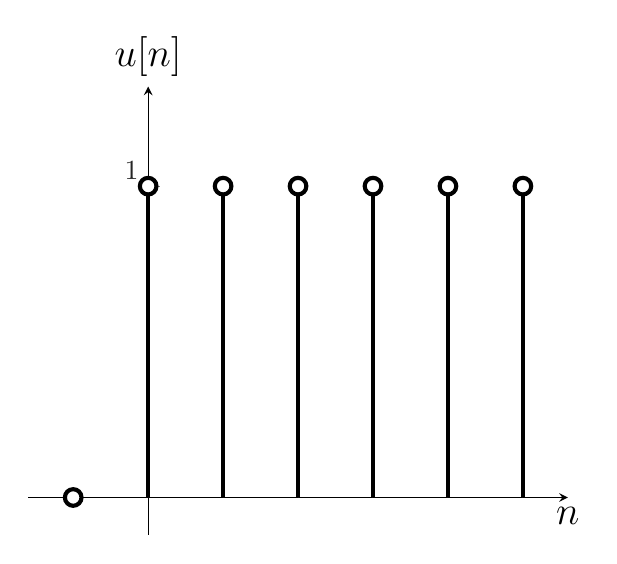
\begin{tikzpicture} 
\begin{axis}[
axis lines*=middle,
enlargelimits = true,
ymin=0,
ymax=1.2,
xmin=-1,
xmax=5,
axis line style={->,>=stealth},
xlabel={\Large $n$},
ylabel={\Large $u[n]$},
yticklabel style = {yshift=0.2cm},
xticklabel style = {yshift=-0.1cm},
every axis x label/.style={
    at={(ticklabel* cs:1)},
    anchor=north,
},
every axis y label/.style={
    at={(ticklabel* cs:1)},
    anchor=south,
},
%xtick=\empty,
ytick={1},
xtick=\empty,
%xtick={-3.14, -1, 1, 3.14},
%xticklabels={$-\pi$, $-\omega_c$, $\omega_c$, $\pi$},
%xmajorgrids,
%ymajorgrids,
every outer y axis line/.append style={white!15!black},
every y tick label/.append style={font=\color{white!15!black}},
legend style={draw=white!15!black,fill=white,legend cell align=left}]

\addplot[ycomb, mark=*, fill=white, mark options={scale=1.5, fill=white}, line width=1.5pt]
  table[row sep=crcr]{%
	-1 	0 \\
	0 	1 \\
	1	1 \\
	2	1 \\
	3	1 \\
	4	1 \\
	5	1 \\
};
\end{axis}
\end{tikzpicture}
}
	\end{column}
\end{columns}
\end{frame}

%
\begin{frame}{Basic sequences}
	
\textbf{Exponential:} $\displaystyle 
x[n] = a^nu[n] = \begin{cases}
a^n, & n \geq 0 \\
0, & \text{otherwise}
\end{cases}$
	
\begin{figure}[h!] 
	\centering 
	\begin{subfigure}[h!]{0.32\textwidth} 
		\resizebox{\linewidth}{!}{\PlotExp{figs/exponential_param.tex}{0.6}{$0 < a < 1$}{0}{2}}
	\end{subfigure}% 
	~ %add desired spacing between images, e. g. ~, \quad, \qquad etc. 
	%(or a blank line to force the subfigure onto a new line) 
	\begin{subfigure}[h!]{0.32\textwidth} 
		\resizebox{\linewidth}{!}{\PlotExp{figs/exponential_param.tex}{1.15}{$a > 1$}{0}{2}}
	\end{subfigure}% 

	\begin{subfigure}[h!]{0.32\textwidth} 
		%\resizebox{\linewidth}{!}{\input{figs/exponential_neg.tex}}
		\resizebox{\linewidth}{!}{\PlotExp{figs/exponential_param.tex}{-0.6}{$-1 < a < 0$}{-2}{2}}
	\end{subfigure}% 
	~ %add desired spacing between images, e. g. ~, \quad, \qquad etc. 
	%(or a blank line to force the subfigure onto a new line) 
	\begin{subfigure}[h!]{0.32\textwidth} 
		\resizebox{\linewidth}{!}{\PlotExp{figs/exponential_param.tex}{-1.15}{$a < -1$}{-2}{2}}
	\end{subfigure}% 
\end{figure}

Exponential exhibits oscillatory behavior for $a < 0$.

Exponential is \textbf{unbounded} if $|a| > 1$.
\end{frame}

%
\begin{frame}{Basic sequences}
	
	\textbf{Sinusoids:} $\displaystyle
	x[n] = \cos(\omega_0 n + \phi)$
	\vspace{-0.2cm}
	\begin{figure}[t!]
		\centering
		\resizebox{0.4\linewidth}{!}{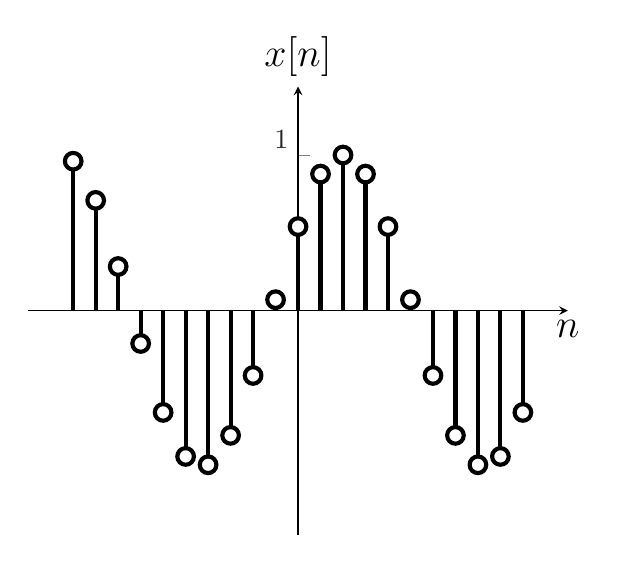
\begin{tikzpicture} 
\begin{axis}[
axis lines*=middle,
enlargelimits = true,
ymin=-1.2,
ymax=1.2,
xmin=-10,
xmax=10,
axis line style={->,>=stealth},
xlabel={\Large $n$},
ylabel={\Large $x[n]$},
yticklabel style = {yshift=0.2cm},
xticklabel style = {yshift=-0.1cm},
every axis x label/.style={
    at={(ticklabel* cs:1)},
    anchor=north,
},
every axis y label/.style={
    at={(ticklabel* cs:1)},
    anchor=south,
},
%xtick=\empty,
ytick={1},
xtick=\empty,
%xtick={-3.14, -1, 1, 3.14},
%xticklabels={$-\pi$, $-\omega_c$, $\omega_c$, $\pi$},
%xmajorgrids,
%ymajorgrids,
every outer y axis line/.append style={white!15!black},
every y tick label/.append style={font=\color{white!15!black}},
legend style={draw=white!15!black,fill=white,legend cell align=left}]

\addplot[ycomb, mark=*, fill=white, mark options={scale=1.5, fill=white}, line width=1.5pt, line width=1.5pt, domain=-10:10, samples=21] {cos(0.5*deg(x -2))};
\end{axis}
\end{tikzpicture}
}
		\label{fig:sinusoid}
	\end{figure}

	Differently from continuous-time sinusoids, discrete-time sinusoids...
	\begin{itemize}
		\item are periodic only if $\omega_0/\pi$ is rational.
		\item have maximum frequency $\omega = \pi$.
	\end{itemize}
	
	\pause	
	\textbf{Complex exponentials:} 
	\begin{equation*}
		e^{j(\omega_0n + \phi)} = \cos(\omega_0 n + \phi) + j\sin(\omega_0 n + \phi) \tag{from Euler's equation}
	\end{equation*}
\end{frame}

%
\begin{frame}{Classification of discrete-time signals}
\begin{block}{Energy and power signals}
	\textbf{Energy signals} have finite energy
	\begin{equation*}
		E = \sum_{n=-\infty}^{\infty} |x[n]|^2
	\end{equation*}
	
	\textbf{Power signals} have infinite energy (e.g., periodic signals), but they have finite average power
	\begin{equation*}
		P = \lim_{N\to\infty}\frac{1}{2N+1}\sum_{n=-N}^{N} |x[n]|^2
	\end{equation*}	
\end{block}	
\end{frame}

%
\begin{frame}{Classification of discrete-time signals}
\begin{block}{Symmetry}
	\begin{equation*}
	x[n] = x[-n] \tag{even symmetry}
	\end{equation*}
	\begin{equation*}
	x[n] = -x[-n] \tag{odd symmetry}
	\end{equation*}
	
	Any signal $x[n]$ can be decomposed as a sum of an even ($x_e[n]$) and an odd ($x_o[n]$) component:
	\begin{equation*}
	x[n] = x_e[n] + x_o[n]
	\end{equation*}	
	where 
	\begin{align}
	x_e[n] = \frac{1}{2}(x[n] + x[-n]) \tag{even component} \\
	x_o[n] = \frac{1}{2}(x[n] - x[-n]) \tag{odd component}
	\end{align}
\end{block}	
\end{frame}

%
\begin{frame}{Discrete-time systems}

\begin{figure}
	\centering
	\resizebox{0.9\linewidth}{!}{\def\layersep{1.5cm}
\def\outsep{0.7cm}
\def\dy{1.25}

\begin{tikzpicture}[->, >=stealth, shorten >= 0pt, draw=black!50, node distance=\layersep, font=\sffamily]
    \tikzstyle{node}=[circle,fill=black,minimum size=2pt,inner sep=0pt]
    \tikzstyle{block}=[draw=black,rectangle,fill=none,minimum size=1.5cm, inner sep=0pt]
    \tikzstyle{annot} = []

	\node[node] (xc) at (0, -\dy cm) {};
    \node[block, text width = 2.7cm, align= center] (DSP) at (2*\layersep, -\dy cm) {Discrete-Time \\ System};
	\coordinate (yc) at (4*\layersep, -\dy cm) {};
		
    \path (xc) edge (DSP);
    \path (DSP) edge (yc);
    
    \node[above = 0.5mm of xc] {$x[n]$};
    \node[above = 0.5mm of yc] {$y[n] = T\{x[n]\}$};
    

\end{tikzpicture}}
	\label{fig:DTsystem}
\end{figure}

\begin{block}{Some important properties}
	\textbf{Linearity or superposition}
	\begin{equation*}
	T\{ax_1[n] + bx_2[n]\} = aT\{x_1[n]\} + bT\{x_2[n]\}
	\end{equation*}
	\textbf{Time invariance or shift invariance}
	\begin{equation*}
	\text{If } d[n] = x[n-n_d], \text{then } T\{d[n]\} = y[n-n_d]
	\end{equation*}
	A time shift of the input causes an equal time shift of the output
\end{block}
\end{frame}

%
\begin{frame}[t]{Linear time-invariant (LTI) systems}
LTI systems are completely characterized by their impulse response.

\begin{figure}
	\centering
	\vspace{-0.25cm}
	\resizebox{0.9\linewidth}{!}{\def\layersep{1.5cm}
\def\outsep{0.7cm}
\def\dy{1.25}

\begin{tikzpicture}[draw=black!50, node distance=\layersep, font=\sffamily]
    \tikzstyle{node}=[circle,fill=black,minimum size=2pt,inner sep=0pt]
    \tikzstyle{block}=[draw=black,rectangle,fill=none,minimum size=1cm, inner sep=0pt]
    \tikzstyle{annot} = []

	\node[node] (xc) at (0, -\dy cm) {};
    \node[block, text width = 2cm, align= center] (DSP) at (2*\layersep, -\dy cm) {LTI System};
	\coordinate (yc) at (4*\layersep, -\dy cm) {};
		
    \path[->, >=stealth, shorten >= 0pt] (xc) edge (DSP);
    \path[->, >=stealth, shorten >= 0pt] (DSP) edge (yc);
    
	\onslide<1|handout:1>{
		\node[block, draw=none, above = 0.5mm of xc, scale=0.5] (tx_signal1) {\resizebox{7cm}{!}{\begin{tikzpicture} 
\begin{axis}[
axis lines*=middle,
enlargelimits = true,
ymin=-1.2,
ymax=1.2,
xmin=-1,
xmax=5,
axis line style={->,>=stealth},
xlabel={\Large $n$},
ylabel={\Large $\delta[n]$},
yticklabel style = {yshift=0.2cm},
xticklabel style = {yshift=-0.1cm},
every axis x label/.style={
    at={(ticklabel* cs:1)},
    anchor=north,
},
every axis y label/.style={
    at={(ticklabel* cs:1)},
    anchor=south,
},
%xtick=\empty,
ytick={1},
xtick=\empty,
%xtick={-3.14, -1, 1, 3.14},
%xticklabels={$-\pi$, $-\omega_c$, $\omega_c$, $\pi$},
%xmajorgrids,
%ymajorgrids,
every outer y axis line/.append style={white!15!black},
every y tick label/.append style={font=\color{white!15!black}},
legend style={draw=white!15!black,fill=white,legend cell align=left}]

\addplot[ycomb, mark=*, fill=white, mark options={scale=1.5, fill=white}, line width=1.5pt]
  table[row sep=crcr]{%
	-1 	0 \\
	0 	1 \\
	1	0 \\
	2	0 \\
	3	0 \\
	4	0 \\
	5	0 \\
};
\end{axis}
\end{tikzpicture}
}};
		\node[below = 0.5mm of xc] {$\delta[n]$};	
		\node[block, draw=none, above = 0.5mm of yc, scale=0.5] (rx_signal1) {\resizebox{7cm}{!}{\begin{tikzpicture} 
\begin{axis}[
axis lines*=middle,
enlargelimits = true,
ymin=-1.2,
ymax=1.2,
xmin=-1,
xmax=5,
axis line style={->,>=stealth},
xlabel={\Large $n$},
ylabel={\Large $h[n]$},
yticklabel style = {yshift=0.2cm},
xticklabel style = {yshift=-0.1cm},
every axis x label/.style={
    at={(ticklabel* cs:1)},
    anchor=north,
},
every axis y label/.style={
    at={(ticklabel* cs:1)},
    anchor=south,
},
%xtick=\empty,
ytick={1},
xtick=\empty,
%xtick={-3.14, -1, 1, 3.14},
%xticklabels={$-\pi$, $-\omega_c$, $\omega_c$, $\pi$},
%xmajorgrids,
%ymajorgrids,
every outer y axis line/.append style={white!15!black},
every y tick label/.append style={font=\color{white!15!black}},
legend style={draw=white!15!black,fill=white,legend cell align=left}]

\addplot[ycomb, mark=*, fill=white, mark options={scale=1.5, fill=white}, line width=1.5pt]
  table[row sep=crcr]{%
	-1 	0 \\
	0 	1 \\
	1	-0.5 \\
	2	0.25 \\
	3  -0.05 \\
	4	0 \\
	5	0 \\
};
\end{axis}
\end{tikzpicture}
}};
		\node[below = 0.5mm of yc] {$h[n]$};
	}

	\onslide<2|handout:2>{
		\node[block, draw=none, above = 0.5mm of xc, scale=0.5] (tx_signal2) {\resizebox{7cm}{!}{\begin{tikzpicture} 
\begin{axis}[
axis lines*=middle,
enlargelimits = true,
ymin=-1.2,
ymax=1.2,
xmin=-1,
xmax=5,
axis line style={->,>=stealth},
xlabel={\Large $n$},
ylabel={\Large $\delta[n-1]$},
yticklabel style = {yshift=0.2cm},
xticklabel style = {yshift=-0.1cm},
every axis x label/.style={
    at={(ticklabel* cs:1)},
    anchor=north,
},
every axis y label/.style={
    at={(ticklabel* cs:1)},
    anchor=south,
},
%xtick=\empty,
ytick={1},
xtick=\empty,
%xtick={-3.14, -1, 1, 3.14},
%xticklabels={$-\pi$, $-\omega_c$, $\omega_c$, $\pi$},
%xmajorgrids,
%ymajorgrids,
every outer y axis line/.append style={white!15!black},
every y tick label/.append style={font=\color{white!15!black}},
legend style={draw=white!15!black,fill=white,legend cell align=left}]

\addplot[ycomb, mark=*, fill=white, mark options={scale=1.5, fill=white}, line width=1.5pt]
  table[row sep=crcr]{%
	-1 	0 \\
	0 	0 \\
	1	1 \\
	2	0 \\
	3	0 \\
	4	0 \\
	5	0 \\
};
\end{axis}
\end{tikzpicture}
}};
		\node[below = 0.5mm of xc] {$\delta[n-1]$};	
		\node[block, draw=none, above = 0.5mm of yc, scale=0.5] (rx_signal2) {\resizebox{7cm}{!}{\begin{tikzpicture} 
\begin{axis}[
axis lines*=middle,
enlargelimits = true,
ymin=-1.2,
ymax=1.2,
xmin=-1,
xmax=5,
axis line style={->,>=stealth},
xlabel={\Large $n$},
ylabel={\Large $h[n-1]$},
yticklabel style = {yshift=0.2cm},
xticklabel style = {yshift=-0.1cm},
every axis x label/.style={
    at={(ticklabel* cs:1)},
    anchor=north,
},
every axis y label/.style={
    at={(ticklabel* cs:1)},
    anchor=south,
},
%xtick=\empty,
ytick={1},
xtick=\empty,
%xtick={-3.14, -1, 1, 3.14},
%xticklabels={$-\pi$, $-\omega_c$, $\omega_c$, $\pi$},
%xmajorgrids,
%ymajorgrids,
every outer y axis line/.append style={white!15!black},
every y tick label/.append style={font=\color{white!15!black}},
legend style={draw=white!15!black,fill=white,legend cell align=left}]

\addplot[ycomb, mark=*, fill=white, mark options={scale=1.5, fill=white}, line width=1.5pt]
  table[row sep=crcr]{%
	-1 	0 \\
	0 	0 \\
	1	1 \\
	2	-0.5 \\
	3  0.25 \\
	4	-0.05 \\
	5	0 \\
};
\end{axis}
\end{tikzpicture}
}};
		\node[below = 0.5mm of yc] {$h[n-1]$};
		\node[below = 2mm of DSP.south] {\textbf{from time invariance}};
	}
	\onslide<3-|handout:3->{
		\node[block, draw=none, above = 0.5mm of xc, scale=0.5] (tx_signal2) {\resizebox{7cm}{!}{\begin{tikzpicture} 
\begin{axis}[
axis lines*=middle,
enlargelimits = true,
ymin=-1.2,
ymax=1.2,
xmin=-1,
xmax=5,
axis line style={->,>=stealth},
xlabel={\Large $n$},
%ylabel={\Large $\delta[n-1]$},
yticklabel style = {yshift=0.2cm},
xticklabel style = {yshift=-0.1cm},
every axis x label/.style={
    at={(ticklabel* cs:1)},
    anchor=north,
},
every axis y label/.style={
    at={(ticklabel* cs:1)},
    anchor=south,
},
%xtick=\empty,
ytick={1},
xtick=\empty,
%xtick={-3.14, -1, 1, 3.14},
%xticklabels={$-\pi$, $-\omega_c$, $\omega_c$, $\pi$},
%xmajorgrids,
%ymajorgrids,
every outer y axis line/.append style={white!15!black},
every y tick label/.append style={font=\color{white!15!black}},
legend style={draw=white!15!black,fill=white,legend cell align=left}]

\addplot[ycomb, mark=*, fill=white, mark options={scale=1.5, fill=white}, line width=1.5pt]
  table[row sep=crcr]{%
	-1 	0 \\
	0 	1 \\
	1	-0.5 \\
	2	0 \\
	3	0 \\
	4	0 \\
	5	0 \\
};
\end{axis}
\end{tikzpicture}
}};
		\node[below = 0.5mm of xc] {$\delta[n] - 0.5\delta[n-1]$};	
		\node[block, draw=none, above = 0.5mm of yc, scale=0.5] (rx_signal2) {\resizebox{7cm}{!}{\begin{tikzpicture} 
\begin{axis}[
axis lines*=middle,
enlargelimits = true,
ymin=-1.2,
ymax=1.2,
xmin=-1,
xmax=5,
axis line style={->,>=stealth},
xlabel={\Large $n$},
%ylabel={\Large $h[n-1]$},
yticklabel style = {yshift=0.2cm},
xticklabel style = {yshift=-0.1cm},
every axis x label/.style={
    at={(ticklabel* cs:1)},
    anchor=north,
},
every axis y label/.style={
    at={(ticklabel* cs:1)},
    anchor=south,
},
%xtick=\empty,
ytick={1},
xtick=\empty,
%xtick={-3.14, -1, 1, 3.14},
%xticklabels={$-\pi$, $-\omega_c$, $\omega_c$, $\pi$},
%xmajorgrids,
%ymajorgrids,
every outer y axis line/.append style={white!15!black},
every y tick label/.append style={font=\color{white!15!black}},
legend style={draw=white!15!black,fill=white,legend cell align=left}]

\addplot[ycomb, mark=*, fill=white, mark options={scale=1.5, fill=white}, line width=1.5pt]
  table[row sep=crcr]{%
	-1 	0 \\
	0 	1 \\
	1	-1 \\
	2	0.5 \\
	3  -0.1750 \\
	4	0.0250 \\
	5	0 \\
};
% 1.0000         0         0    0.0750   -0.0250
\end{axis}
\end{tikzpicture}
}};
		\node[below = 0.5mm of yc] {$h[n] - 0.5h[n-1]$};
	}
	\onslide<3|handout:3>{\node[below = 2mm of DSP.south] {\textbf{from linearity}};}

\end{tikzpicture}}
	\label{fig:DTimp}
\end{figure}
\vspace{-0.5cm}
\onslide<4-|handout:4>{
\begin{block}{The convolution sum}
	\begin{equation*}
		y[n] = \sum_{k=-\infty}^{\infty} x[k]h[n-k] = \sum_{k=-\infty}^{\infty} x[n-k]h[k]
	\end{equation*}
	Shorthand notation: $y[n] = x[n]\ast h[n]$ or $ y[n] = (x\ast h)[n]$
\end{block}
}

\end{frame}

\begin{frame}{Other properties of discrete-time systems}

\begin{block}{Memoryless}
	A system is \textbf{memoryless} if its output at time $n$, $y[n]$,  depends only on the present input $x[n]$.
\end{block}

\begin{block}{Causality}
	A system is \textbf{causal} if its output at time $n$, $y[n]$, depends only on the present and past samples of the input $\{x[n], x[n-1], x[n-2], \ldots\}$. All physical systems are causal.
	\vspace{0.5cm}
	
	For \textbf{LTI systems}, causality implies $h[n] = 0, n < 0$
	\begin{equation*}\tag{Convolution sum for causal systems}
	y[n] = \sum_{\tikz[baseline]{
			\node[fill=blue!20,anchor=base] (t1) {$k=0$};}}^{\infty} x[n-k]h[k] = \sum_{k=-\infty}^{n} x[k]h[n-k]
	\end{equation*}
	
\end{block}

\end{frame}

\begin{frame}{Other properties of discrete-time systems}
	
	\begin{block}{Stability}
		A system is \textbf{BIBO stable} if every bounded input ($|x[n]| < B_x < \infty$) produces a bounded output ($|y[n]| < B_y < \infty$)

		\vspace{0.25cm}
		For \textbf{LTI systems},
		\vspace{-0.25cm}
		\begin{align*}
		|y[n]| &= \bigg|\sum_{k = -\infty}^{\infty} x[n-k]h[k]\bigg| \tag{Convolution sum} \\
		&\leq \sum_{k = -\infty}^{\infty} |x[n-k]||h[k]| \tag{Triangle inequality} \\
		& \leq B_x\sum_{k = -\infty}^{\infty} |h[k]| \tag{Bounded input $|x[n]| < B_x < \infty$} \\
		& < B_y < \infty \tag{only if $\displaystyle\sum_{k=-\infty}^{\infty}|h[k]| < \infty$}
		\end{align*}
		\vspace{-0.3cm}
		 
		 Therefore, an LTI system is BIBO stable only if its impulse response $h[k]$ is \textbf{absolute summable}.
	\end{block}
\end{frame}


%
\begin{frame}<beamer:0>{Classify the following discrete-time systems}
	\centering
	\resizebox{\linewidth}{!}{
		\begin{tabular}{M{4cm}|c|c|c|c|c}
			\hline
			\textbf{System} & \textbf{Linear} & \textbf{Time invariant} & \textbf{Memoryless} & \textbf{Causal} & \textbf{BIBO stable} \\[2ex]
			\hline
			\makecell{Constant offset \\ $y[n] = x[n] + C, C \neq 0$} & & & & &  \\[3ex]
			\hline
			\makecell{Time shift \\ $y[n] = x[n-n_d]$} & & & & & \\[3ex]	
			\hline
			\makecell{Squaring \\ $y[n] = x^2[n]$} & & & & & \\[3ex]
			\hline
			\makecell{Accumulator \\ $y[n] = \displaystyle\sum_{k=-\infty}^nx[k]$} & & & & & \\[3ex]
			\hline
			\makecell{Compressor \\ $y[n] = x[Mn], M > 1$} & & & & & \\[3ex]
			\hline
			\makecell{Differentiator \\ $y[n] = x[n] - x[n-1]$} & & & & & \\[3ex]
			\hline
			\makecell{A difference equation \\ $y[n] = x[n] + y[n-1]$} & & & & & \\[3ex]
			\hline
		\end{tabular}
	}
\end{frame}

%
\begin{frame}<handout:0>{Classify the following discrete-time systems}
\centering
\resizebox{\linewidth}{!}{
	\begin{tabular}{M{4cm}|c|c|c|c|c}
		\hline
		\textbf{System} & \textbf{Linear} & \textbf{Time invariant} & \textbf{Memoryless} & \textbf{Causal} & \textbf{BIBO stable} \\[2ex]
		\hline
		\makecell{Constant offset \\ $y[n] = x[n] + C, C \neq 0$} & \onslide<2->{N} & \onslide<2->{Y} & \onslide<2->{Y} & \onslide<2->{Y} & \onslide<2->{Y} \\[3ex]
		\hline
		\makecell{Time shift \\ $y[n] = x[n-n_d]$} & \onslide<3->{Y} & \onslide<3->{Y} & \onslide<3->{N, if $n_d \neq 0$} & \onslide<3->{Y, if $n_d > 0$} & \onslide<3->{Y} \\[3ex]	
		\hline
		\makecell{Squaring \\ $y[n] = x^2[n]$} & \onslide<4->{N} & \onslide<4->{Y} & \onslide<4->{Y} & \onslide<4->{Y} & \onslide<4->{Y} \\[3ex]
		\hline
		\makecell{Accumulator \\ $y[n] = \displaystyle\sum_{k=-\infty}^nx[k]$} & \onslide<5->{Y} & \onslide<5->{Y} & \onslide<5->{N} & \onslide<5->{Y} & \onslide<5->{N} \\[3ex]
		\hline
		\makecell{Compressor \\ $y[n] = x[Mn], M > 1$} & \onslide<6->{Y} & \onslide<6->{N} & \onslide<6->{N} & \onslide<6->{N} & \onslide<6->{Y} \\[3ex]
		\hline
		\makecell{Differentiator \\ $y[n] = x[n] - x[n-1]$} & \onslide<7->{Y} & \onslide<7->{Y} & \onslide<7->{N} & \onslide<7->{Y} & \onslide<7->{Y} \\[3ex]
		\hline
		\makecell{A difference equation \\ $y[n] = x[n] + y[n-1]$} & \onslide<8->{Y} & \onslide<8->{Y} & \onslide<8->{N} & \onslide<8->{Y} & \onslide<8->{N} \\[3ex]
		\hline
	\end{tabular}
}
\end{frame}

\subsection{The Discrete-Time Fourier Transform}
%
\begin{frame}{Frequency-domain representation of LTI systems}

Output of an LTI system to a complex exponential 

\vspace{-0.5cm}
\begin{columns}[t]
	\begin{column}{0.3\textwidth}
		\begin{center}
			\begin{tikzpicture}[->, >=stealth, shorten >= 0pt, draw=black!50, node distance=0.6\textwidth]
			\tikzstyle{node}=[circle,fill=black,minimum size=2pt,inner sep=0pt]
			\tikzstyle{block}=[draw=black,rectangle,fill=none,minimum size=1cm, inner sep=0pt]
			\tikzstyle{annot} = []
			
			\node[node] (xc) at (0, 0 cm) {};
			\node[block, right of=xc, text width = 2cm, align= center] (DSP) {LTI System};
			\coordinate[right of=DSP] (yc) {};
			
			\path (xc) edge (DSP);
			\path (DSP) edge (yc);
			
			\node[above = 0.5mm of xc] {$x[n] = e^{j\omega n}$};			
			\end{tikzpicture}
		\end{center}
	\end{column}
	\begin{column}{0.8\textwidth}
		\begin{align*}
		y[n] &= \sum_{k=-\infty}^{\infty} h[k]e^{j\omega(n-k)}  \\
		&= \underbrace{\bigg(\sum_{k=-\infty}^{\infty} h[k]e^{-j\omega k}\bigg)}_\text{$H(e^{j\omega})$}e^{j\omega n} = H(e^{j\omega})e^{j\omega n}
		\end{align*}
	\end{column}
\end{columns}	
		
\begin{itemize}
	\pause\item $H(e^{j\omega})$ only depends on the impulse response of the LTI system
	\pause\item The output of an LTI system to a complex exponential is a complex exponential of same frequency, but with possibly different amplitude and phase
\end{itemize}

\pause
\begin{block}{Conclusions}
	\begin{itemize}
		\item Complex exponentials are \textbf{eigenfunctions} of LTI systems, and $H(e^{j\omega})$ are the corresponding eigenvalues.
		\item By representing signals as a sum of complex exponentials, we can readily calculate their output to an LTI system: $Y(e^{j\omega}) = H(e^{j\omega})X(e^{j\omega})$
	\end{itemize} 
\end{block}
\end{frame}

%
\begin{frame}{Discrete-time Fourier transform (DTFT)}

\begin{block}{Definition}
\begin{equation} \tag{Direct transform}
X(e^{j\omega}) = \sum_{n=-\infty}^{\infty} x[n]e^{-j\omega n} 
\end{equation}

\begin{equation}\tag{Inverse transform}
x[n] = \frac{1}{2\pi}\int_{-\pi}^{\pi}X(e^{j\omega})e^{j\omega n}d\omega
\end{equation}
\end{block}

\textbf{Important:}
\begin{itemize}
	\item The DTFT is periodic with period $2\pi$: $\displaystyle X(e^{j(\omega + 2\pi)}) = X(e^{j\omega})$
	\item If $x[n]$ is \textbf{absolute summable} i.e., $\sum_{k=-\infty}^{\infty} |x[k]| < \infty$, then the DTFT exists. This is a \textit{sufficient} condition, but it is \textit{not a necessary} condition.
	\item Absolute summability also implies that the DTFT \textbf{converges uniformly} to a continuous function of $\omega$.
\end{itemize}
\end{frame}

%
\begin{frame}[t]{Example: the ideal lowpass filter}

\begin{columns}[t]
	\begin{column}{0.5\linewidth}
		\textbf{Time domain}
		\vspace{0.1cm}
		\begin{equation*}
			h_{lpf}[n] = \frac{\sin\omega_cn}{\pi n} = \frac{\omega_c}{\pi}\mathrm{sinc}\Big(\frac{\omega_c}{\pi} n\Big)
		\end{equation*}
	\end{column}

	\begin{column}{0.5\linewidth}
		\textbf{Frequency domain}
		\vspace{-0.2cm}
		\only<1|handout:1>{
		\begin{equation*}
			H_{lpf}(e^{j\omega}) = \begin{cases}
			1, & |\omega|\leq\omega_c \\
			0, & \omega_c < |\omega|\leq \pi
			\end{cases}
		\end{equation*}	
		}
		\only<2-|handout:2->{
			\begin{equation*}
			H_{M}(e^{j\omega}) = \sum_{n=\tikz[baseline]{
					\node[fill=blue!20,anchor=base,scale=0.7] {$-M$};
			}}^{\tikz[baseline]{
			\node[fill=blue!20,anchor=base,scale=0.7] {$M$};
		}} \frac{\sin\omega_cn}{\pi n}e^{-j\omega n}
			\end{equation*}	
		}
	\end{column}
\end{columns}
\vspace{0.3cm}

\centering
\resizebox{\linewidth}{!}{\begin{tikzpicture} 
\only<1|handout:1>{
\begin{axis}[
name=ideal_lpf_td,
anchor=origin,
axis lines*=middle,
enlargelimits = true,
ymin=-0.1,
ymax=1.2*0.5,
xmin=-10,
xmax=10,
axis line style={->,>=stealth},
xlabel={$n$},
ylabel={$h_{lpf}[n]$},
yticklabel style = {yshift=0.2cm},
xticklabel style = {yshift=-0.1cm},
every axis x label/.style={
	at={(ticklabel* cs:1)},
	anchor=north,
},
every axis y label/.style={
	at={(ticklabel* cs:1)},
	anchor=south,
},
ytick=0.5,
yticklabels={$\frac{\omega_c}{\pi}$},
xtick=\empty,
every outer y axis line/.append style={white!15!black},
every y tick label/.append style={font=\color{white!15!black}},
legend style={draw=white!15!black,fill=white,legend cell align=left}]

\addplot[ycomb, mark=*, fill=white, mark options={scale=1.5, fill=white}, line width=1.5pt, domain=-10:10, samples=21] {sin(deg(pi/2*x))/(pi*x) + 1/2*(x == 0)};
\addplot[smooth, black!20, line width=1pt, domain=-10:10, samples=21] {sin(deg(pi/2*x))/(pi*x) + 1/2*(x == 0)};
\end{axis}

\begin{axis}[
name=ideal_lpf_fd,
at=(ideal_lpf_td.right of south east), anchor=left of south west,
axis lines*=middle,
enlargelimits = true,
xmax=4,
xmin=-4,
ymin=-0.2,
ymax=1.2,
axis line style={->,>=stealth},
xlabel={$\omega$},
ylabel={$H_{lpf}(e^{j\omega})$},
yticklabel style = {yshift=0.2cm},
xticklabel style = {yshift=-0.3cm},
every axis x label/.style={
    at={(ticklabel* cs:1)},
    anchor=north,
},
every axis y label/.style={
    at={(ticklabel* cs:1)},
    anchor=south,
},
xtick=\empty,
ytick={1},
xtick={-3.14, -1.5708, 1.5708, 3.14},
xticklabels={$-\pi$, $-\omega_c$, $\omega_c$, $\pi$},
every outer y axis line/.append style={white!15!black},
every y tick label/.append style={font=\color{white!15!black}},
legend style={draw=white!15!black,fill=white,legend cell align=left}]

	\addplot[black, domain=-pi/2:pi/2, samples=2,line width=2pt] {1};
	\addplot[black, line width=2pt] coordinates {(-pi/2, 0) (-pi/2, 1.01)};
	\addplot[black, domain=-pi:-pi/2, samples=2,line width=2pt] {0};
	\addplot[black, domain=pi/2:pi, samples=2,line width=2pt] {0};
	\addplot[black, line width=2pt] coordinates {(pi/2, 0) (pi/2, 1.01)};
\end{axis}
}

%%%%%%%%%%%%%%%%%% 
\only<2|handout:2>{
	\begin{axis}[
	name=truncated_lpf_td,
	anchor=origin,
	axis lines*=middle,
	enlargelimits = true,
	ymin=-0.1,
	ymax=1.2*0.5,
	xmin=-7,
	xmax=7,
	axis line style={->,>=stealth},
	xlabel={$n$},
	ylabel={$h_{lpf}[n]$},
	yticklabel style = {yshift=0.2cm},
	xticklabel style = {yshift=0.6cm},
	every axis x label/.style={
		at={(ticklabel* cs:1)},
		anchor=north,
	},
	every axis y label/.style={
		at={(ticklabel* cs:1)},
		anchor=south,
	},
	ytick=0.5,
	yticklabels={$\frac{\omega_c}{\pi}$},
	xtick={-7, 7},
	xticklabels={\tikz[baseline]{\node[fill=blue!20,anchor=base,scale=0.7] {$-M$};}, \tikz[baseline]{\node[fill=blue!20,anchor=base,scale=0.7] {$M$};}},
	every outer y axis line/.append style={white!15!black},
	every y tick label/.append style={font=\color{white!15!black}},
	legend style={draw=white!15!black,fill=white,legend cell align=left}]
	
	\addplot[ycomb, mark=*, fill=white, mark options={scale=1.5, fill=white}, line width=1.5pt, domain=-7:7, samples=15] {sin(deg(pi/2*x))/(pi*x) + 1/2*(x == 0)};
	\addplot[smooth, black!20, line width=1pt, domain=-7:7, samples=15] {sin(deg(pi/2*x))/(pi*x) + 1/2*(x == 0)};
	\end{axis}
	
	\begin{axis}[
	name=truncated_lpf_fd,
	at=(truncated_lpf_td.right of south east), anchor=left of south west,
	axis lines*=middle,
	enlargelimits = true,
	xmax=4,
	xmin=-4,
	ymin=-0.2,
	ymax=1.2,
	axis line style={->,>=stealth},
	xlabel={$\omega$},
	ylabel={$H_{lpf}(e^{j\omega})$},
	yticklabel style = {yshift=0.2cm},
	xticklabel style = {yshift=-0.3cm},
	every axis x label/.style={
		at={(ticklabel* cs:1)},
		anchor=north,
	},
	every axis y label/.style={
		at={(ticklabel* cs:1)},
		anchor=south,
	},
	xtick=\empty,
	ytick={1},
	xtick={-3.14, -1.5708, 1.5708, 3.14},
	xticklabels={$-\pi$, $-\omega_c$, $\omega_c$, $\pi$},
	every outer y axis line/.append style={white!15!black},
	every y tick label/.append style={font=\color{white!15!black}},
	legend style={draw=white!15!black,fill=white,legend cell align=left}]
	
	\addplot[black!20, domain=-pi/2:pi/2, samples=2,line width=2pt] {1};
	\addplot[black!20, line width=2pt] coordinates {(-pi/2, 0) (-pi/2, 1.01)};
	\addplot[black!20, domain=-pi:-pi/2, samples=2,line width=2pt] {0};
	\addplot[black!20, domain=pi/2:pi, samples=2,line width=2pt] {0};
	\addplot[black!20, line width=2pt] coordinates {(pi/2, 0) (pi/2, 1.01)};
	
	\addplot [color=black, solid, line width=1.5pt, forget plot]
	table[row sep=crcr]{
		-3.1416 0.039209 \\
		-3.0781 0.034184 \\
		-3.0147 0.020324 \\
		-2.9512 0.00099044 \\
		-2.8877 -0.019066 \\
		-2.8243 -0.0348 \\
		-2.7608 -0.042056 \\
		-2.6973 -0.038583 \\
		-2.6339 -0.024655 \\
		-2.5704 -0.0031491 \\
		-2.5069 0.020968 \\
		-2.4435 0.041656 \\
		-2.38 0.053128 \\
		-2.3165 0.051242 \\
		-2.2531 0.034652 \\
		-2.1896 0.0054863 \\
		-2.1261 -0.030621 \\
		-2.0627 -0.065184 \\
		-1.9992 -0.088127 \\
		-1.9357 -0.089437 \\
		-1.8723 -0.060929 \\
		-1.8088 0.0022081 \\
		-1.7453 0.10035 \\
		-1.6819 0.22911 \\
		-1.6184 0.37975 \\
		-1.5549 0.54037 \\
		-1.4915 0.69762 \\
		-1.428 0.83864 \\
		-1.3645 0.95293 \\
		-1.3011 1.0338 \\
		-1.2376 1.0793 \\
		-1.1741 1.0921 \\
		-1.1107 1.0788 \\
		-1.0472 1.0487 \\
		-0.98373 1.0122 \\
		-0.92026 0.97863 \\
		-0.8568 0.95526 \\
		-0.79333 0.94598 \\
		-0.72986 0.95114 \\
		-0.6664 0.96788 \\
		-0.60293 0.99105 \\
		-0.53947 1.0146 \\
		-0.476 1.0328 \\
		-0.41253 1.0417 \\
		-0.34907 1.0397 \\
		-0.2856 1.0278 \\
		-0.22213 1.0093 \\
		-0.15867 0.98893 \\
		-0.0952 0.97181 \\
		-0.031733 0.96207 \\
		0.031733 0.96207 \\
		0.0952 0.97181 \\
		0.15867 0.98893 \\
		0.22213 1.0093 \\
		0.2856 1.0278 \\
		0.34907 1.0397 \\
		0.41253 1.0417 \\
		0.476 1.0328 \\
		0.53947 1.0146 \\
		0.60293 0.99105 \\
		0.6664 0.96788 \\
		0.72986 0.95114 \\
		0.79333 0.94598 \\
		0.8568 0.95526 \\
		0.92026 0.97863 \\
		0.98373 1.0122 \\
		1.0472 1.0487 \\
		1.1107 1.0788 \\
		1.1741 1.0921 \\
		1.2376 1.0793 \\
		1.3011 1.0338 \\
		1.3645 0.95293 \\
		1.428 0.83864 \\
		1.4915 0.69762 \\
		1.5549 0.54037 \\
		1.6184 0.37975 \\
		1.6819 0.22911 \\
		1.7453 0.10035 \\
		1.8088 0.0022081 \\
		1.8723 -0.060929 \\
		1.9357 -0.089437 \\
		1.9992 -0.088127 \\
		2.0627 -0.065184 \\
		2.1261 -0.030621 \\
		2.1896 0.0054863 \\
		2.2531 0.034652 \\
		2.3165 0.051242 \\
		2.38 0.053128 \\
		2.4435 0.041656 \\
		2.5069 0.020968 \\
		2.5704 -0.0031491 \\
		2.6339 -0.024655 \\
		2.6973 -0.038583 \\
		2.7608 -0.042056 \\
		2.8243 -0.0348 \\
		2.8877 -0.019066 \\
		2.9512 0.00099044 \\
		3.0147 0.020324 \\
		3.0781 0.034184 \\
		3.1416 0.039209 \\
	};
	
	\node at (axis cs: 3.14, 1.1) {\Large \tikz[baseline]{
			\node[fill=blue!20,anchor=base] (t1) {$M = 7$}}};
	
	\end{axis}
}

%%%%%%%%%%%%%%%%%% 
\only<3|handout:3>{
	\begin{axis}[
	name=truncated_lpf_td,
	anchor=origin,
	axis lines*=middle,
	enlargelimits = true,
	ymin=-0.1,
	ymax=1.2*0.5,
	xmin=-19,
	xmax=19,
	axis line style={->,>=stealth},
	xlabel={$n$},
	ylabel={$h_{lpf}[n]$},
	yticklabel style = {yshift=0.2cm},
	xticklabel style = {yshift=0.6cm},
	every axis x label/.style={
		at={(ticklabel* cs:1)},
		anchor=north,
	},
	every axis y label/.style={
		at={(ticklabel* cs:1)},
		anchor=south,
	},
	ytick=0.5,
	yticklabels={$\frac{\omega_c}{\pi}$},
	xtick={-19, 19},
	xticklabels={\tikz[baseline]{\node[fill=blue!20,anchor=base,scale=0.7] {$-M$};}, \tikz[baseline]{\node[fill=blue!20,anchor=base,scale=0.7] {$M$};}},
	every outer y axis line/.append style={white!15!black},
	every y tick label/.append style={font=\color{white!15!black}},
	legend style={draw=white!15!black,fill=white,legend cell align=left}]
	
	\addplot[ycomb, mark=*, fill=white, mark options={scale=1.5, fill=white}, line width=1.5pt,  domain=-19:19, samples=39] {sin(deg(pi/2*x))/(pi*x) + 1/2*(x == 0)};
	\addplot[smooth, black!20, line width=1pt, domain=-19:19, samples=39] {sin(deg(pi/2*x))/(pi*x) + 1/2*(x == 0)};
	\end{axis}
	
	\begin{axis}[
	name=truncated_lpf_fd,
	at=(truncated_lpf_td.right of south east), anchor=left of south west,
	axis lines*=middle,
	enlargelimits = true,
	xmax=4,
	xmin=-4,
	ymin=-0.2,
	ymax=1.2,
	axis line style={->,>=stealth},
	xlabel={$\omega$},
	ylabel={$H_{lpf}(e^{j\omega})$},
	yticklabel style = {yshift=0.2cm},
	xticklabel style = {yshift=-0.3cm},
	every axis x label/.style={
		at={(ticklabel* cs:1)},
		anchor=north,
	},
	every axis y label/.style={
		at={(ticklabel* cs:1)},
		anchor=south,
	},
	xtick=\empty,
	ytick={1},
	xtick={-3.14, -1.5708, 1.5708, 3.14},
	xticklabels={$-\pi$, $-\omega_c$, $\omega_c$, $\pi$},
	every outer y axis line/.append style={white!15!black},
	every y tick label/.append style={font=\color{white!15!black}},
	legend style={draw=white!15!black,fill=white,legend cell align=left}]
	
	\addplot[black!20, domain=-pi/2:pi/2, samples=2,line width=2pt] {1};
	\addplot[black!20, line width=2pt] coordinates {(-pi/2, 0) (-pi/2, 1.01)};
	\addplot[black!20, domain=-pi:-pi/2, samples=2,line width=2pt] {0};
	\addplot[black!20, domain=pi/2:pi, samples=2,line width=2pt] {0};
	\addplot[black!20, line width=2pt] coordinates {(pi/2, 0) (pi/2, 1.01)};
	
	\addplot [color=black, solid, line width=1.5pt, forget plot]
table[row sep=crcr]{
	-3.1416 0.015876 \\
	-3.11 0.012806 \\
	-3.0784 0.0047726 \\
	-3.0469 -0.0051424 \\
	-3.0153 -0.013122 \\
	-2.9837 -0.01607 \\
	-2.9521 -0.012801 \\
	-2.9206 -0.0045107 \\
	-2.889 0.0056547 \\
	-2.8574 0.013781 \\
	-2.8259 0.016676 \\
	-2.7943 0.013113 \\
	-2.7627 0.0043342 \\
	-2.7311 -0.006365 \\
	-2.6996 -0.014863 \\
	-2.668 -0.017776 \\
	-2.6364 -0.013789 \\
	-2.6048 -0.0042266 \\
	-2.5733 0.0073679 \\
	-2.5417 0.016523 \\
	-2.5101 0.019535 \\
	-2.4785 0.014937 \\
	-2.447 0.0041704 \\
	-2.4154 -0.0088347 \\
	-2.3838 -0.019057 \\
	-2.3522 -0.022276 \\
	-2.3207 -0.016768 \\
	-2.2891 -0.004133 \\
	-2.2575 0.011106 \\
	-2.226 0.023056 \\
	-2.1944 0.026652 \\
	-2.1628 0.019706 \\
	-2.1312 0.0040161 \\
	-2.0997 -0.01496 \\
	-2.0681 -0.029875 \\
	-2.0365 -0.034159 \\
	-2.0049 -0.024686 \\
	-1.9734 -0.0034348 \\
	-1.9418 0.022586 \\
	-1.9102 0.043309 \\
	-1.8786 0.049014 \\
	-1.8471 0.034142 \\
	-1.8155 0.00025733 \\
	-1.7839 -0.042935 \\
	-1.7523 -0.079062 \\
	-1.7208 -0.08885 \\
	-1.6892 -0.055218 \\
	-1.6576 0.031713 \\
	-1.6261 0.1712 \\
	-1.5945 0.35111 \\
	-1.5629 0.55018 \\
	-1.5313 0.74274 \\
	-1.4998 0.90461 \\
	-1.4682 1.0186 \\
	-1.4366 1.0783 \\
	-1.405 1.0884 \\
	-1.3735 1.0631 \\
	-1.3419 1.0211 \\
	-1.3103 0.98084 \\
	-1.2787 0.95576 \\
	-1.2472 0.95147 \\
	-1.2156 0.96573 \\
	-1.184 0.99043 \\
	-1.1524 1.0152 \\
	-1.1209 1.0311 \\
	-1.0893 1.0336 \\
	-1.0577 1.0234 \\
	-1.0261 1.0055 \\
	-0.99457 0.98732 \\
	-0.963 0.97552 \\
	-0.93143 0.97388 \\
	-0.89985 0.98214 \\
	-0.86828 0.99648 \\
	-0.83671 1.0111 \\
	-0.80513 1.0206 \\
	-0.77356 1.0217 \\
	-0.74198 1.0146 \\
	-0.71041 1.0024 \\
	-0.67884 0.98987 \\
	-0.64726 0.98183 \\
	-0.61569 0.98105 \\
	-0.58412 0.98748 \\
	-0.55254 0.99841 \\
	-0.52097 1.0095 \\
	-0.48939 1.0166 \\
	-0.45782 1.0172 \\
	-0.42625 1.0111 \\
	-0.39467 1.001 \\
	-0.3631 0.99079 \\
	-0.33152 0.98432 \\
	-0.29995 0.98398 \\
	-0.26838 0.98979 \\
	-0.2368 0.99942 \\
	-0.20523 1.0091 \\
	-0.17366 1.0152 \\
	-0.14208 1.0154 \\
	-0.11051 1.0096 \\
	-0.078934 1.0002 \\
	-0.047361 0.99075 \\
	-0.015787 0.98491 \\
	0.015787 0.98491 \\
	0.047361 0.99075 \\
	0.078934 1.0002 \\
	0.11051 1.0096 \\
	0.14208 1.0154 \\
	0.17366 1.0152 \\
	0.20523 1.0091 \\
	0.2368 0.99942 \\
	0.26838 0.98979 \\
	0.29995 0.98398 \\
	0.33152 0.98432 \\
	0.3631 0.99079 \\
	0.39467 1.001 \\
	0.42625 1.0111 \\
	0.45782 1.0172 \\
	0.48939 1.0166 \\
	0.52097 1.0095 \\
	0.55254 0.99841 \\
	0.58412 0.98748 \\
	0.61569 0.98105 \\
	0.64726 0.98183 \\
	0.67884 0.98987 \\
	0.71041 1.0024 \\
	0.74198 1.0146 \\
	0.77356 1.0217 \\
	0.80513 1.0206 \\
	0.83671 1.0111 \\
	0.86828 0.99648 \\
	0.89985 0.98214 \\
	0.93143 0.97388 \\
	0.963 0.97552 \\
	0.99457 0.98732 \\
	1.0261 1.0055 \\
	1.0577 1.0234 \\
	1.0893 1.0336 \\
	1.1209 1.0311 \\
	1.1524 1.0152 \\
	1.184 0.99043 \\
	1.2156 0.96573 \\
	1.2472 0.95147 \\
	1.2787 0.95576 \\
	1.3103 0.98084 \\
	1.3419 1.0211 \\
	1.3735 1.0631 \\
	1.405 1.0884 \\
	1.4366 1.0783 \\
	1.4682 1.0186 \\
	1.4998 0.90461 \\
	1.5313 0.74274 \\
	1.5629 0.55018 \\
	1.5945 0.35111 \\
	1.6261 0.1712 \\
	1.6576 0.031713 \\
	1.6892 -0.055218 \\
	1.7208 -0.08885 \\
	1.7523 -0.079062 \\
	1.7839 -0.042935 \\
	1.8155 0.00025733 \\
	1.8471 0.034142 \\
	1.8786 0.049014 \\
	1.9102 0.043309 \\
	1.9418 0.022586 \\
	1.9734 -0.0034348 \\
	2.0049 -0.024686 \\
	2.0365 -0.034159 \\
	2.0681 -0.029875 \\
	2.0997 -0.01496 \\
	2.1312 0.0040161 \\
	2.1628 0.019706 \\
	2.1944 0.026652 \\
	2.226 0.023056 \\
	2.2575 0.011106 \\
	2.2891 -0.004133 \\
	2.3207 -0.016768 \\
	2.3522 -0.022276 \\
	2.3838 -0.019057 \\
	2.4154 -0.0088347 \\
	2.447 0.0041704 \\
	2.4785 0.014937 \\
	2.5101 0.019535 \\
	2.5417 0.016523 \\
	2.5733 0.0073679 \\
	2.6048 -0.0042266 \\
	2.6364 -0.013789 \\
	2.668 -0.017776 \\
	2.6996 -0.014863 \\
	2.7311 -0.006365 \\
	2.7627 0.0043342 \\
	2.7943 0.013113 \\
	2.8259 0.016676 \\
	2.8574 0.013781 \\
	2.889 0.0056547 \\
	2.9206 -0.0045107 \\
	2.9521 -0.012801 \\
	2.9837 -0.01607 \\
	3.0153 -0.013122 \\
	3.0469 -0.0051424 \\
	3.0784 0.0047726 \\
	3.11 0.012806 \\
	3.1416 0.015876 \\
};
	
	\node at (axis cs: 3.14, 1.1) {\Large \tikz[baseline]{
			\node[fill=blue!20,anchor=base] (t1) {$M = 19$}}};
	
	\end{axis}
}

\end{tikzpicture}}
\end{frame}

%
\begin{frame}{Convergence of the DTFT}
\begin{itemize}
	\item The sinc function is not absolute summable, but it is \textbf{square summable}
	\begin{equation*}
		\sum_{n=-\infty}^{\infty} |\mathrm{sinc}(n)|^2 < \infty
	\end{equation*}
	\item In this case, the DTFT does not converge uniformly; it converges in the mean-square sense
	\item The oscillations are known as \textbf{Gibbs phenomenon}, and they occur whenever there is a discontinuity in the frequency domain
	\item Interestingly, as $M\to\infty$ the oscillations become more rapid, but the size of the ripples does not decrease
	\item The DTFT may exist even when sequences are neither absolute summable nor square summable. Examples: a constant, unit step, complex exponentials
	\item Although all this may seem like a mathematical curiosity, it has important implications in filter design. More on this in lecture 9.
\end{itemize}
	
\end{frame}

%
\begin{frame}{DTFT properties}
\begin{itemize}
\item Linearity
	\begin{equation*}
	ax_1[n]  + bx_2[n] \Longleftrightarrow aX_1(e^{j\omega})+bX_2(e^{j\omega})
	\end{equation*}
\item Time shift, delay for $n_d > 0$, advance for $n_d < 0$
	\begin{equation*}
	x[n-n_d] \Longleftrightarrow e^{-j\omega n_d}X(e^{j\omega})
	\end{equation*}
\item Frequency shift (modulation)
	\begin{equation*}
	e^{j\omega_0n}x[n] \Longleftrightarrow X(e^{j(\omega-\omega_0)})
	\end{equation*}
\item Convolution
	\begin{equation*}
	y[n] = x[n]\ast h[n] \Longleftrightarrow Y(e^{j\omega}) = X(e^{j\omega})H(e^{j\omega})
	\end{equation*}
\item Multiplication of sequences (windowing)
	\begin{equation*}
	x[n]w[n] \Longleftrightarrow \frac{1}{2\pi}\int_{-\pi}^{\pi}X(e^{j\theta})W(e^{j(\omega-\theta)}){d\theta}
	\end{equation*}
\end{itemize}
\end{frame}

%
\begin{frame}{DTFT properties}
\begin{itemize}
	\item Linear weighting
		\begin{equation*}
		nx[n] \Longleftrightarrow j\frac{dX(e^{j\omega})}{d\omega}
		\end{equation*}
	\item Time reversal
		\begin{equation*}
		x[-n] \Longleftrightarrow X(e^{-j\omega})
		\end{equation*}
	\item Parseval's theorem
		\begin{equation*}
		\sum_{n=-\infty}^{\infty}x[n]y^*[n] = \frac{1}{2\pi}\int_{-\pi}^{\pi}X(e^{j\omega})Y^*(e^{j\omega})\mathrm{d}\omega
		\end{equation*}
		if $x[n] = y[n]$
		\begin{equation*}\tag{signal energy}
		\sum_{n=-\infty}^{\infty}|x[n]|^2 = \frac{1}{2\pi}\int_{-\pi}^{\pi}|X(e^{j\omega})|^2\mathrm{d}\omega
		\end{equation*}	
	\item Deterministic autocorrelation function
		\begin{equation*}
		c_{xx}[n] = \sum_{m=-\infty}^{\infty}x[m]x[n+m] \Longleftrightarrow X(e^{j\omega})X^*(e^{j\omega}) = |X(e^{j\omega})|^2
		\end{equation*}	
\end{itemize}
\end{frame}

%
\subsection{The $z$-Transform}

\begin{frame}{The $z$-Transform}

The $z$-transform is a generalization of the DTFT and it is applicable to a broader class of signals and systems.

\begin{block}{Definition}
	\begin{equation} \tag{Direct transform}
	X(z) = \sum_{n=-\infty}^{\infty} x[n]z^{-n} 
	\end{equation}
	
	\begin{equation}\tag{Inverse transform}
	x[n] = \frac{1}{2j\pi}\oint_{\mathcal{C}}X(z)z^{n-1}\mathrm{d}z
	\end{equation}
\end{block}

\begin{itemize}
	\item The $z$-transform has a \textbf{region of convergence (ROC)}, which is the values of $z$ for which the infinite sum in the direct transform is finite. Without the ROC, the $z$-transform is an \textbf{ambiguous representation} of a signal.
	\item The inverse transform is given by the contour integral over some complex path $\mathcal{C}$. This is generally laborious, so we'll obtain the inverse $z$-transform through indirect methods such as \textbf{partial fraction expansion}.
\end{itemize}
\end{frame}

%
\begin{frame}{The $z$-Transform}
$x[n] = z^n, z\in\mathbb{C}$ is another \textbf{eigenfunction} of LTI systems

\textit{Proof:}
\begin{align*}
y[n] &= \sum_{k=-\infty}^{\infty} h[k]z^{(n-k)} \tag{from convolution sum} \\
&= \bigg(\sum_{k=-\infty}^{\infty} h[k]z^{-k}\bigg)z^{n} \tag{rearranging}\\
&= H(z)z^{n} \tag{By definition $H(z) \equiv \sum_{k=-\infty}^{\infty} h[k]z^{-k}$}
\end{align*}	

\begin{itemize}
	\item We can always write $z^n = r^ne^{j\omega n}$ (polar coordinates)
	\item The eigenfunction $e^{j\omega n}$, used in the DTFT, is just a particular case ($r=1$) of the eigenfunction used in the $z$-transform
	\item The factor $r^n$ helps the $z$-transform sum converge to a broader class of signals
\end{itemize}

\end{frame}

%
\begin{frame}{Relation between DTFT and the $z$-Transform}

\begin{columns}[t]
	\begin{column}{0.5\textwidth}
		\begin{block}{DTFT}
			\vspace{-0.5cm}
			\begin{equation} \tag{Direct transform}
			X(e^{j\omega}) = \sum_{n=-\infty}^{\infty} x[n]\tikz[baseline]{
				\node[fill=blue!20,anchor=base] (t1) {$e^{-j\omega n}$};
			}
			\end{equation}
		\end{block}
	\end{column}
	\begin{column}{0.5\textwidth}
		\begin{block}{$z$-Transform}
			\vspace{-0.2cm}
			\begin{equation} \tag{Direct transform}
			X(z) = \sum_{n=-\infty}^{\infty} x[n]\tikz[baseline]{
				\node[fill=blue!20,anchor=base] (t1) {$z^{-n}$};
			}
			\end{equation}
		\end{block}
	\end{column}
\end{columns}
\vspace{0.4cm}
\begin{itemize}
	\pause\item The DTFT is equal to the $z$-transform evaluated on the unit circle
	\item DTFT is periodic with period $2\pi$.
	\pause\item \textbf{Question:} Does the DTFT exist if the ROC of the $z$-transform does not include the unit circle?
\end{itemize}

\vspace{-0.4cm}
\flushright
\resizebox{0.35\linewidth}{!}{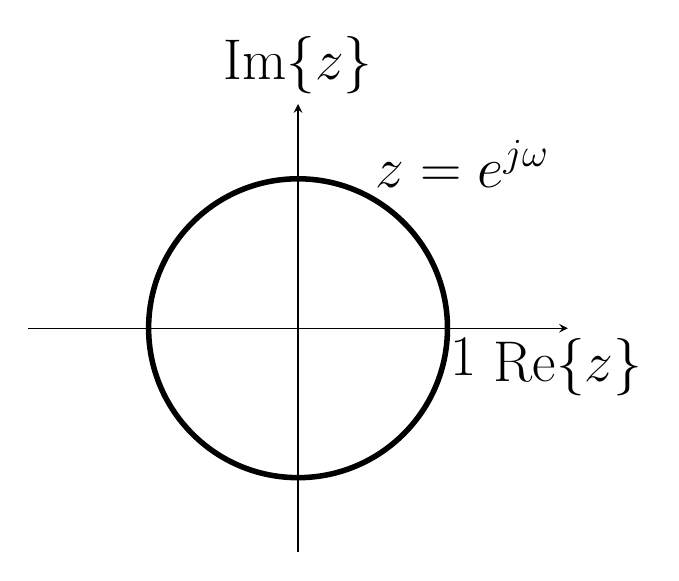
\begin{tikzpicture} 
\begin{axis}[
axis equal,
axis lines*=middle,
enlargelimits = false,
xmax=1.5,
xmin=-1.5,
ymin=-1.5,
ymax=1.5,
axis line style={->,>=stealth},
xlabel={\huge $\mathrm{Re}\{z\}$},
ylabel={\huge $\mathrm{Im}\{z\}$},
every axis x label/.style={
    at={(ticklabel* cs:1)},
    anchor=north,
},
every axis y label/.style={
    at={(ticklabel* cs:1)},
    anchor=south,
},
xtick={1},
ytick=\empty,
xticklabels={\huge 1},
%xmajorgrids,
%ymajorgrids,
xticklabel style = {xshift=+0.2cm},
every outer y axis line/.append style={white!15!black},
every y tick label/.append style={font=\color{white!15!black}},
legend style={draw=white!15!black,fill=white,legend cell align=left}]
\draw[black, line width=2pt] (axis cs:0,0) circle [radius=1];
\node (z) at (axis cs: 1.1, 1.1) {\huge $z = e^{j\omega}$};
\end{axis}
\end{tikzpicture}
}
\end{frame}

%
\begin{frame}{For what will we use the $z$-transform?}
	\begin{enumerate}
		\item Representing LTI systems
		\item Determining stability of LTI systems
		\item Finding frequency response of stable systems
		\item Solving difference equations
	\end{enumerate}
\end{frame}


%
\begin{frame}{Rational $z$-transforms}
	
Rational $z$-transforms are a ratio of two polynomials in $z^{-1}$ (or $z$)
\begin{align*}
	X(z) &= \frac{B(z)}{A(z)} = \frac{b_0 + b_1z^{-1}+\ldots+b_Mz^{-M}}{a_0 + a_1z^{-1}+\ldots+a_Nz^{-N}} \\
	&= \frac{b_0}{a_0}z^{N-M}\frac{(z-z_1)(z-z_2)\ldots(z-z_M)}{(z-p_1)(z-p_2)\ldots(z-p_N)}
\end{align*}
\begin{itemize}
	\pause\item The \textbf{zeros} of a $z$-transform are the values of $z$ for which $X(z) = 0$
	\pause\item The \textbf{poles} of a $z$-transform are the values of $z$ for which $X(z) = \infty$. By definition, the ROC cannot contain any pole
	\pause\item $X(z)$ has $M$ zeros $\{z_1, z_2, \ldots, z_M\}$, which are the roots of the numerator polynomial $B(z)$
	\pause\item $X(z)$ has $N$ poles $\{p_1, p_2, \ldots, p_M\}$, which are the roots of the denominator polynomial $A(z)$
	\pause\item If $N-M > 0$, $X(z)$ has more $N-M$ zeros at $z = 0$
	\pause\item If $N-M < 0$, $X(z)$ has more $M-N$ poles at $z = 0$
	\pause\item If the coefficients $\{b_0, \ldots, b_M\}, \{a_0, \ldots, a_N\}$ are real, the poles and zeros are either real or they appear in complex conjugate pairs
\end{itemize}	
\end{frame}

%
\begin{frame}{Examples}

\begin{block}{1. Right-sided exponential $x[n] = a^nu[n]$}

\begin{equation*} 
X(z) = \sum_{n=0}^\infty a^nz^{-n} = \sum_{n=0}^\infty (az^{-1})^n 
\end{equation*}
This sum converges only if $|az^{-1}| < 1$. Hence, ROC: $|z| > |a|$.
~\\
~\\
\begin{columns}
	\begin{column}{0.5\textwidth}
		From the sum of an infinite geometric progression:
		\begin{equation*} 
		X(z) = \frac{1}{1-az^{-1}} = \frac{z}{z-a}
		\end{equation*}
		Pole at $z = a$ and zero at $z = 0$.
		~\\
		~\\
		The ROC of a causal signal is the \textbf{exterior of a circle} whose radius is the magnitude of the outermost pole $|a|$.
	\end{column}
	\begin{column}{0.5\textwidth}  %%<--- here
		\begin{figure}
			\centering
			\resizebox{0.95\linewidth}{!}{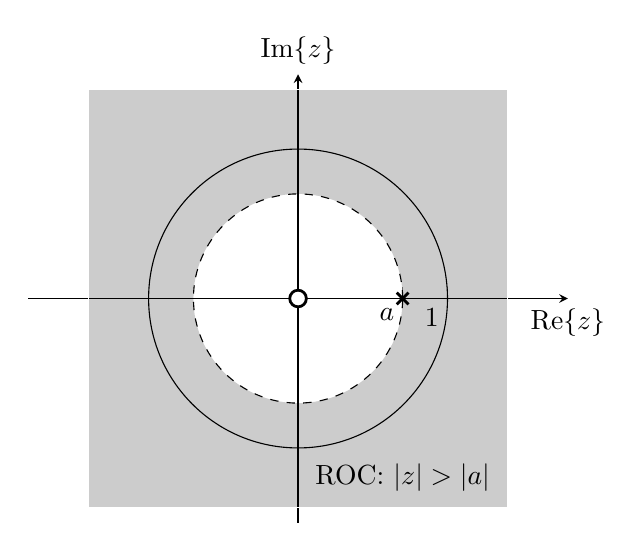
\begin{tikzpicture} 
\begin{axis}[
axis equal,
axis lines*=middle,
enlargelimits = false,
xmax=1.5,
xmin=-1.5,
ymin=-1.5,
ymax=1.5,
axis line style={->,>=stealth},
xlabel={$\mathrm{Re}\{z\}$},
ylabel={$\mathrm{Im}\{z\}$},
every axis x label/.style={
    at={(ticklabel* cs:1)},
    anchor=north,
},
every axis y label/.style={
    at={(ticklabel* cs:1)},
    anchor=south,
},
xtick={0.7, 1},
ytick=\empty,
xticklabels={$a$, 1},
%xmajorgrids,
%ymajorgrids,
xticklabel style = {xshift=-0.2cm},
every outer y axis line/.append style={white!15!black},
every y tick label/.append style={font=\color{white!15!black}},
legend style={draw=white!15!black,fill=white,legend cell align=left}]
\addplot[line width=1pt,mark=*, mark size = 3pt, mark options={fill=white}] coordinates {(0, 0)};
\addplot[line width=1pt,mark=x, mark size = 3pt] coordinates {(0.7, 0)};
\draw (axis cs:0,0) circle [black, line width=2pt, radius=1];
\draw[name path=A, dashed] (axis cs:0,0) circle [black, line width=2pt, radius=0.7];
\draw [name path=B, white] (axis cs:-1.4, -1.4) rectangle (axis cs:1.4,1.4);
%\draw[fill=black!20] (axis cs:1.3, -1.3) rectangle (axis cs:1.5,-1.1);
\addplot [
thick,
color=black,
fill=black, 
fill opacity=0.2
]
fill between[
of=A and B,
];
\node[fill=black!20] (roc) at (axis cs:0.7, -1.2) {ROC: $|z| > |a|$};
\end{axis}
\end{tikzpicture}
}
			\label{fig:right_sided_exp}
		\end{figure}
	\end{column}
\end{columns}

\end{block}
\end{frame}

%
\begin{frame}{Examples}
\begin{block}{2. Left-sided exponential $x[n] = -a^nu[-n-1]$}
	\begin{equation*} 
	X(z) = -\sum_{n=-\infty}^{-1} a^nz^{-n} = -\sum_{n=1}^{\infty} a^{-n}z^{n} = 1-\sum_{n=0}^{\infty} (a^{-1}z)^{n}
	\end{equation*}
	
	This sum converges only if $|a^{-1}z| < 1$. Hence, ROC: $|z| < |a|$.
	
	\begin{columns}
		\begin{column}{0.6\textwidth}
			Once again from the sum of an infinite geometric progression:
			\begin{equation*} 
				X(z) = \frac{1}{1-az^{-1}} = \frac{z}{z-a}\tag{\textbf{Same as before!}}
			\end{equation*}
			~\\
			Without the ROC, the $z$-transform is an \textbf{ambiguous representation} of a signal.
			~\\
			~\\
			The ROC of an anti-causal signal is the \textbf{interior of a circle} whose radius is the magnitude of the innermost pole $|a|$.
		\end{column}
		\begin{column}{0.4\textwidth}  %%<--- here
			\resizebox{1.18\linewidth}{!}{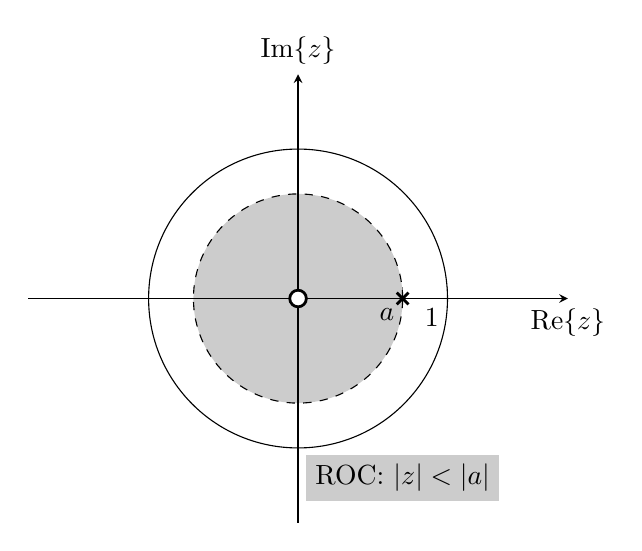
\begin{tikzpicture} 
\begin{axis}[
axis equal,
axis lines*=middle,
enlargelimits = false,
xmax=1.5,
xmin=-1.5,
ymin=-1.5,
ymax=1.5,
axis line style={->,>=stealth},
xlabel={$\mathrm{Re}\{z\}$},
ylabel={$\mathrm{Im}\{z\}$},
every axis x label/.style={
    at={(ticklabel* cs:1)},
    anchor=north,
},
every axis y label/.style={
    at={(ticklabel* cs:1)},
    anchor=south,
},
xtick={0.7, 1},
ytick=\empty,
xticklabels={$a$, 1},
%xmajorgrids,
%ymajorgrids,
xticklabel style = {xshift=-0.2cm},
every outer y axis line/.append style={white!15!black},
every y tick label/.append style={font=\color{white!15!black}},
legend style={draw=white!15!black,fill=white,legend cell align=left}]
\addplot[line width=1pt,mark=*, mark size = 3pt, mark options={fill=white}] coordinates {(0, 0)};
\addplot[line width=1pt,mark=x, mark size = 3pt] coordinates {(0.7, 0)};
\draw (axis cs:0,0) circle [black, line width=2pt, radius=1];
\draw[name path=A, dashed] (axis cs:0,0) circle [black, line width=2pt, radius=0.7];
\draw[name path=O, dashed] (axis cs:0,0) circle [black, line width=2pt, radius=0.01];
\addplot [
thick,
color=black,
fill=black, 
fill opacity=0.2
]
fill between[
of=O and A,
];
\node[fill=black!20] (roc) at (axis cs:0.7, -1.2) {ROC: $|z| < |a|$};
\end{axis}
\end{tikzpicture}
}
		\end{column}
	\end{columns}
	
\end{block}
\end{frame}

\begin{frame}{Examples}

\begin{block}{3. Two-sided exponential $x[n] = -b^nu[-n-1] + a^nu[n]$}
	We can use the previous results and the linearity property of the $z$-transform:
	\vspace{-0.25cm}
	\begin{align*} 
	X(z) &= -\sum_{n=-\infty}^{-1} b^nz^{-n} + \sum_{n=0}^\infty a^nz^{-n} = \frac{1}{1-bz^{-1}} + \frac{1}{1-az^{-1}} 
	\end{align*}
	
	The ROC is the intersection of the two previous ROCs because both sums must exist. Therefore:
	ROC: $|b| < |z| < |a|$.

	\begin{columns}
		\begin{column}{0.5\textwidth}
			Assuming $a = -1/3$ and $b=1/2$
			\begin{equation*} 
			X(z) = \frac{2z(z-1/12)}{(z+1/3)(z-1/2)}
			\end{equation*}
			Poles at $z = -1/3, 1/2$\\
			Zeros at $z = 0, 1/12$
			~\\
			~\\
			The ROC of a two-sided signal is an \textbf{annulus} (ring-shaped region).
			
		\end{column}
		\begin{column}{0.5\textwidth}  %%<--- here
			\begin{figure}
				\centering
				\resizebox{0.95\linewidth}{!}{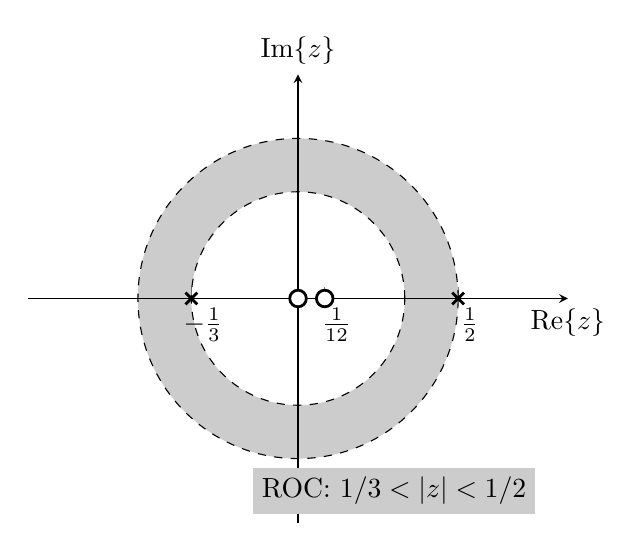
\begin{tikzpicture} 
\begin{axis}[
axis equal,
axis lines*=middle,
enlargelimits = false,
xmax=0.7,
xmin=-0.7,
ymin=-0.7,
ymax=0.7,
axis line style={->,>=stealth},
xlabel={$\mathrm{Re}\{z\}$},
ylabel={$\mathrm{Im}\{z\}$},
every axis x label/.style={
    at={(ticklabel* cs:1)},
    anchor=north,
},
every axis y label/.style={
    at={(ticklabel* cs:1)},
    anchor=south,
},
xtick={-0.3333, 0, 0.0833, 0.5},
ytick=\empty,
xticklabels={$-\frac{1}{3}$, 0, $\frac{1}{12}$, $\frac{1}{2}$},
xticklabel style = {xshift=0.15cm},
every outer y axis line/.append style={white!15!black},
every y tick label/.append style={font=\color{white!15!black}},
legend style={draw=white!15!black,fill=white,legend cell align=left}]
\addplot[line width=1pt,mark=*, only marks, mark size = 3pt, mark options={fill=white}] coordinates {(0, 0) (1/12, 0)};
\addplot[line width=1pt,mark=x, only marks, mark size = 3pt] coordinates {(0.5, 0) (-0.3333, 0)};
%\draw (axis cs:0,0) circle [black, line width=2pt, radius=1];
\draw[name path=A, dashed] (axis cs:0,0) circle [black, line width=2pt, radius=1/3];
\draw[name path=O, dashed] (axis cs:0,0) circle [black, line width=2pt, radius=1/2];
\addplot [
thick,
color=black,
fill=black, 
fill opacity=0.2
]
fill between[
of=O and A,
];
\node[fill=black!20] (roc) at (axis cs:0.3, -0.6) {ROC: $1/3 < |z| < 1/2$};
\end{axis}
\end{tikzpicture}
}
				\label{fig:left_sided_exp}
			\end{figure}
		\end{column}
	\end{columns}
	
\end{block}
\end{frame}

%
\begin{frame}{Properties of the region of convergence}
	The ROC tells a lot about a signal or system
	\begin{enumerate}
		\item If the ROC is the exterior of a circle (ROC = $\{|z| > |a|\}$), the system/signal is \textbf{causal}, where $a$ is the outermost pole. The ROC cannot contain any pole
		\pause\item If a \textbf{LTI system is BIBO stable} (i.e., $\sum_{n=-\infty}^{\infty} |h[n]|<\infty$), the ROC must contain the unit circle.
		
		\textit{Proof:}
		\vspace{-0.25cm}
		\begin{align*}
		|H(z)| &= \bigg|\sum_{n=-\infty}^{\infty}h[n]z^{-n}\bigg| \\
		&\leq \sum_{n=-\infty}^{\infty} |h[n]||z|^{-n} \tag{From triangle inequality} \\
		&= \sum_{n=-\infty}^{\infty} |h[n]| <\infty \tag{$z = e^{j\omega} \implies |z|=1$}
		\end{align*}
		\pause\item A \textbf{causal and stable LTI system} has all poles inside the unit circle. This follows from the first two properties.
	\end{enumerate}
\end{frame}

%
\begin{frame}{Properties of the $z$-transform}
\resizebox{\linewidth}{!}{
\begin{tabular}{p{3cm}|l|l|p{3.5cm}}
	\hline
	Property & Time-Domain & z-Domain & ROC \\
	\hline
	~ & $x[n]$ & $X(z)$ & ROC = $\{r_2 < |z| < r_1\}$ \\
	Notation & $x_1[n]$ & $X_1(z)$ & ROC$_1$ \\
	~ & $x_2[n]$ & $X_2(z)$ & ROC$_2$ \\
	Linearity & $a_1x_1[n] + a_2x_2[n]$ & $a_1X_1(z) + a_2X_2(z)$ & at least $\mathrm{ROC}_1 \cap \mathrm{ROC}_2$ \\
	Time shifting & $x[n-k]$ & $X(z)z^{-k}$ & $\mathrm{ROC}-\begin{cases}\{0\}, k > 0 \\\{\infty\}, k < 0\\\end{cases}$ \\
	Scaling in the $z$-domain & $a^nx[n]$ & $X(\frac{z}{a})$ & $|ar_1| < |z| < |ar_2|$ \\
	Time reversal & $x[-n]$ & $X(z^{-1})$ & $|\frac{1}{r_1}| < |z| < |\frac{1}{r_2}|$ \\
	Conjugation & $x[n]^{*}$ & $X(z^{*})^{*}$ & ROC \\
	Real part & Re$\{x[n]\}$ & $\frac{X(z) + X(z^{*})^{*}}{2}$ & includes ROC \\
	Imaginary part & Im$\{x[n]\}$ & $\frac{X(z) - X(z^{*})^{*}}{2}$ & includes ROC \\
	Differentiation in the $z$-domain & $nx[n]$ & $-z\frac{\mathrm{d}X(z)}{\mathrm{d}z}$ & ROC \\
	Convolution & $x_1[n]\ast x_2[n]$ & $X_1(z)\cdot X_2(z)$ & at least $\mathrm{ROC}_1\cap \mathrm{ROC}_2$ \\
	Correlation & $x_1[n]\ast x_2[-n]$ & $X_1(z)\cdot X_2(z^{-1})$ & at least $\mathrm{ROC}_1\cap \mathrm{ROC}_2(z^{-1})$ \\
	Initial value theorem & for $x[n]$ casual & $x[0] = \lim_{z\to\infty} X(z)$ \\
	\hline
\end{tabular}
}
\end{frame}

%
\begin{frame}{Inverse $z$-transform}
\begin{itemize}
	\item We generally don't use the inverse $z$-transform contour integral
	\item It's typically much easier to use indirect methods such as \textbf{partial fraction expansion}
	\item The goal is to write the $z$-transform as a sum of simpler $z$-transforms for which the inverse is tabulated
\end{itemize}
\vspace{-0.25cm}
\begin{align*}
X(z) &= \frac{B(z)}{A(z)} = \frac{b_0 + b_1z^{-1}+\ldots+b_Mz^{-M}}{a_0 + a_1z^{-1}+\ldots+a_Nz^{-N}} \tag{$z$-transform we want to invert} \\
&= \frac{r_1}{1-p_1z^{-1}} + \ldots + \frac{r_N}{1-p_Nz^{-1}} + k_1 + \ldots + k_{M-N+1}z^{-(M-N)} \tag{sum of simpler $z$-transforms}
\end{align*}
The equation above assumes all poles are different.

\begin{itemize}
	\item $\{r_1,\ldots,r_N\}$ are known as the residues
	\item $\{p_1,\ldots,p_N\}$ are the poles
	\item $\{k_1, \ldots, k_{M-N+1}\}$ are the direct terms. The direct terms are only present if $M > N$
\end{itemize}

\end{frame}

%
\begin{frame}{Inverse $z$-transform}

Suppose that the $l$th pole of $X(z)$ has \textbf{multiplicity} $m$ (the pole is repeated $m$ times). In this case, the partial fraction expansion must also include the terms
~\\

\begin{equation*}
\frac{r_l}{1-p_lz^{-1}} + \frac{r_{l+1}}{(1-p_lz^{-1})^2} + \ldots + \frac{r_{l+m-1}}{(1-p_lz^{-1})^l}
\end{equation*}
~\\
~\\
How to obtain $\{r_1,\ldots,r_N\}$, $\{p_1,\ldots,p_N\}$, and $\{k_1 + \ldots + k_{M-N+1}\}$?
\begin{itemize}
	\item Analytically
	\item Matlab function \href{https://www.mathworks.com/help/signal/ref/residuez.html}{\texttt{residuez}}
\end{itemize}

\end{frame}

\subsection{Difference Equations}
%
\begin{frame}{Linear constant-coefficient difference equation}
	Many practical problems appear in the form of difference equations
	\begin{equation*}
		\sum_{k=0}^N a_k y[n-k] = \sum_{k=0}^Mb_k x[n-k]
	\end{equation*}
	\pause This difference equation defines an LTI system only if:
	\begin{enumerate}
		\item All coefficients $a_k, b_k$ are constant
		\item The initial conditions (or \textit{rest} conditions) are zero $y[-N] = y[-N+1] =\ldots=y[-1] = 0$
	\end{enumerate}	 
	
	\pause Applying the linearity and time-shift properties of the $z$-transform:
	\begin{align*}
		\sum_{k=0}^N a_kY(z)z^{-k} = \sum_{k=0}^M b_kX(z)z^{-k} \\
		H(z) = \frac{Y(z)}{X(z)} = \frac{\sum_{k=0}^M b_kz^{-k}}{\sum_{k=0}^N a_kz^{-jk}}
	\end{align*}
	
	$H(z)$ is a \textbf{rational $z$-transform}.
\end{frame}

\begin{frame}{Example: first-order system}
	\textbf{First-order system:} $y[n] - ay[n-1] = x[n]$
	~\\
	~\\
	Calculating the $z$-transform:
	\begin{align*}
	Y(z) - aY(z)z^{-1} &= X(z) \\
	Y(z)(1 - az^{-1}) &= X(z) \\
	H(z) = \frac{Y(z)}{X(z)} &= \frac{1}{1 - az^{-1}} 
	\end{align*}
	
	\begin{itemize}
		\pause\item This corresponds to the exponential: $h[n] = a^nu[n]$.\\ \textbf{Questions:} Why the causal exponential? 
		For what values of $a$ is this system stable?
		\pause\item This system is \textbf{autoregressive} i.e., the present output depends on previous outputs
		\pause\item Autoregressive systems have \textbf{infinite impulse response (IIR)}
		\pause\item Systems with rational $z$-transforms with non-zero poles are IIR
	\end{itemize}
	
\end{frame}

\begin{frame}
\vspace{0.5cm}
Let's assume $a =0.5$, then $y[n] - 0.5y[n-1] = x[n]$
\begin{align*}
	H(z) = \frac{1}{1 - 0.5z^{-1}} \xrightarrow{z = e^{j\omega}} H(e^{j\omega}) = \frac{1}{1 - 0.5e^{-j\omega}} 
\end{align*}

In Matlab:\\
$> \mathtt{freqz(1, [1, -0.5])}$

\begin{center}
	\begin{tikzpicture}
	\node (img1) {\resizebox{0.65\linewidth}{!}{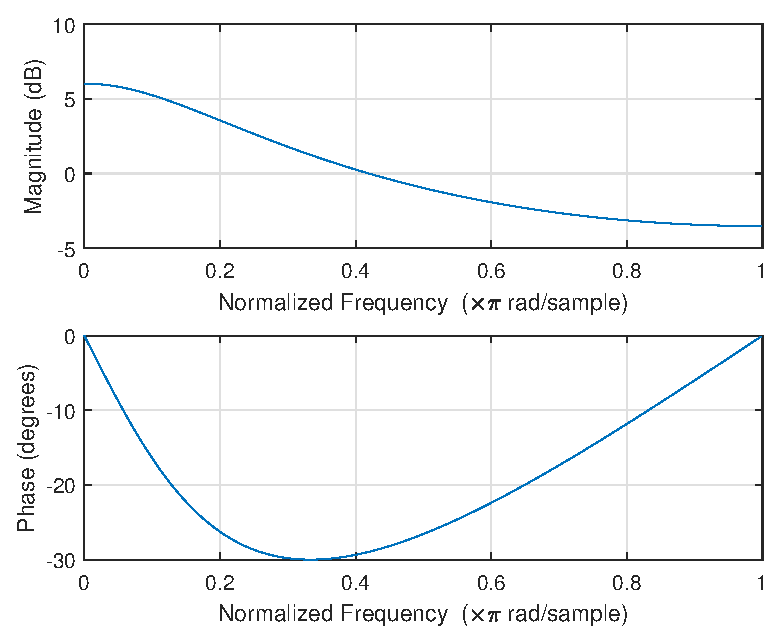
\includegraphics{figs/first_order_sys_freqz.eps}}};
	\node at ($(img1.north east) -(4cm, 0.75cm)$) {$20\log_{10}(|H(e^{j\omega})|)$};
	\node at ($(img1.east)-(4cm, 1cm)$) {$\angle H(e^{j\omega}) = \arg(H(e^{j\omega}))$};
	\end{tikzpicture}
\end{center}

\end{frame}


\begin{frame}{Example: moving average system}
\textbf{Moving average:} $y[n] = \frac{1}{M}(x[n] + x[n-1] + x[n-2] + \ldots+ x[n-M+1])$
~\\
~\\

Calculating the $z$-transform:
\begin{align*}
Y(z) &= \frac{1}{M}X(z)(1 + z^{-1} + \ldots+ z^{-(n-M+1)}) \\
H(z) = \frac{Y(z)}{X(z)} &= \frac{1}{M}(1 + z^{-1} + \ldots+ z^{-(n-M+1)})
\end{align*}	

\begin{itemize}
	\pause\item This system has impulse response $h[n] = 1/M(\delta[n] + \delta[n-1] + \ldots + \delta[n-M+1])$
	\pause\item The impulse response only depends on a finite number of previous inputs. Hence, this system has a \textbf{finite impulse response (FIR)}
\end{itemize}	
\end{frame}

\begin{frame}
\vspace{0.5cm}
Let's assume $M = 4$, then $y[n] = \frac{1}{4}(x[n] + x[n-1] + x[n-2] + x[n-3])$
\begin{align*}
H(z) = \frac{1}{4}(1 + z^{-1} + \ldots + z^{-3}) \xrightarrow{z = e^{j\omega}} H(e^{j\omega}) = \frac{1}{4}(1 + e^{-j\omega} + \ldots+ e^{-3j\omega})
\end{align*}

In Matlab:\\
$> \mathtt{freqz([1, 1, 1, 1]/4, 1)}$

\begin{center}
	\resizebox{0.65\linewidth}{!}{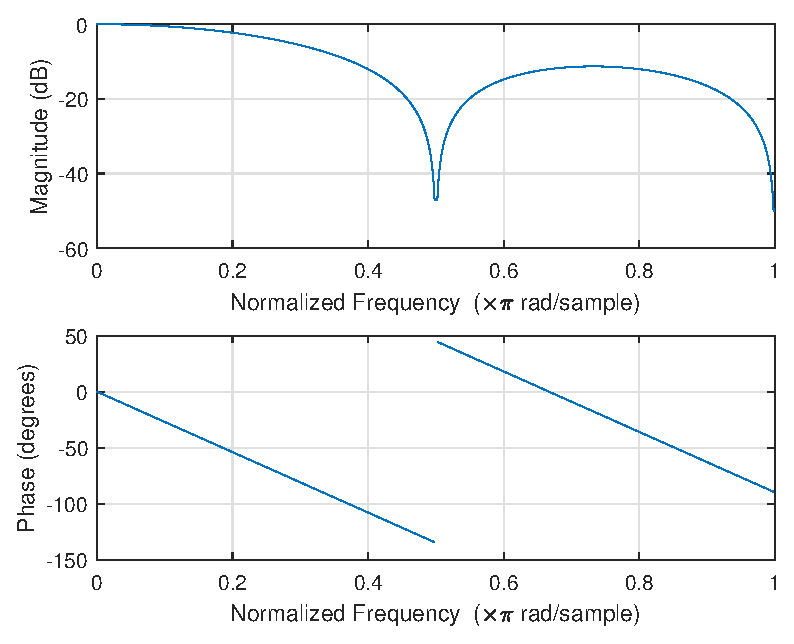
\includegraphics{figs/moving_avg4_freqz.eps}}
\end{center}

\end{frame}

\begin{frame}{Example: output of a moving average filter}

\onslide<1-2|handout:1> {Suppose the input signal frequency is $\omega_0 = 0.2\pi$}

\onslide<3-4|handout:2> {What would happen if $\omega_0 = 0.5\pi$?}

\begin{center}
	\resizebox{\linewidth}{!}{\def\layersep{3cm}
\def\outsep{0.7cm}
\def\dy{1.25}

\begin{tikzpicture}[draw=black!50, node distance=\layersep, font=\sffamily]
    \tikzstyle{node}=[circle,fill=black,minimum size=2pt,inner sep=0pt]
    \tikzstyle{block}=[draw=black,rectangle,fill=none,minimum size=1cm, inner sep=0pt]
    \tikzstyle{annot} = []

	\node[node] (xc) at (0, 0 cm) {};
    \node[block, text width = 2cm, align= center, right of=xc] (DSP) {$h[n], H(z)$};
	\coordinate[right of=DSP] (yc) {};
		
    \path[->, >=stealth, shorten >= 0pt] (xc) edge (DSP);
    \path[->, >=stealth, shorten >= 0pt] (DSP) edge (yc);
    
	\onslide<1-2|handout:1>{
		\node[block, draw=none, scale=0.5] (tx_signal1) at ($(xc.north) + (-1.5cm, 3cm)$) {\resizebox{12cm}{!}{\begin{tikzpicture}
\begin{axis}[
width=4.52in,
height=3.56in,
scale only axis,
separate axis lines,
every outer x axis line/.append style={white!15!black},
every x tick label/.append style={font=\color{white!15!black}},
xmin=0.00,
xmax=20.00,
ymin=-1.00,
ymax=1.00,
xlabel={},
ylabel={},
xmajorgrids,
ymajorgrids,
every outer y axis line/.append style={white!15!black},
every y tick label/.append style={font=\color{white!15!black}},
legend style={draw=white!15!black,fill=white,legend cell align=left}]
\definecolor{matlabColor1}{rgb}{0.000000,0.000000,1.000000}
\addplot [color=matlabColor1, only marks, line width=1.5pt, mark=*, mark size=2pt, forget plot]
table[row sep=crcr]{
	0 1 \\
	1 6.1232e-17 \\
	2 -1 \\
	3 -1.837e-16 \\
	4 1 \\
	5 3.0616e-16 \\
	6 -1 \\
	7 -4.2863e-16 \\
	8 1 \\
	9 5.5109e-16 \\
	10 -1 \\
	11 -2.4499e-15 \\
	12 1 \\
	13 -9.8034e-16 \\
	14 -1 \\
	15 -2.6948e-15 \\
	16 1 \\
	17 -7.3541e-16 \\
	18 -1 \\
	19 -2.9398e-15 \\
	20 1 \\
};

\end{axis}
\end{tikzpicture}}};
		\node[below = 0.5mm of xc] {$x[n] = \cos(\omega_0n)$};	
		\node[below = 0.5mm of yc] {$y[n] = x[n]\ast h[n]$};
	}
	\onslide<2|handout:1>{
		\node[block, draw=none, scale=0.5] (rx_signal1) at ($(yc.north) + (1.5cm, 3cm)$) {\resizebox{12cm}{!}{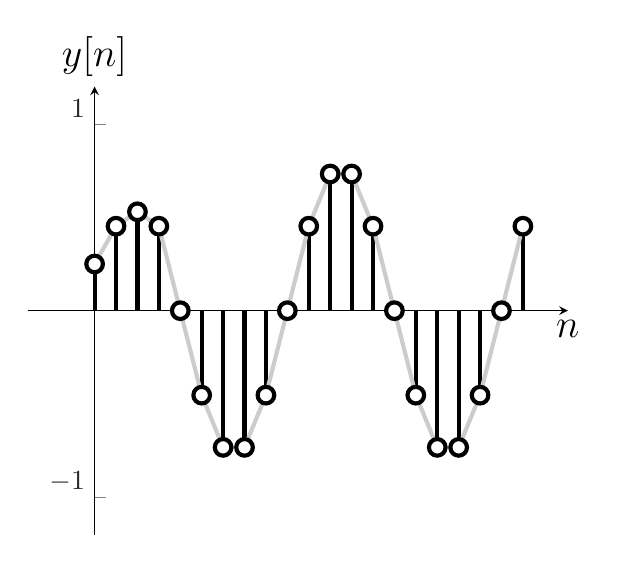
\begin{tikzpicture}
\begin{axis}[
axis lines*=middle,
enlargelimits = true,
ymin=-1,
ymax=1,
xmin=-1,
xmax=20,
axis line style={->,>=stealth},
xlabel={\Large $n$},
ylabel={\Large $y[n]$},
yticklabel style = {yshift=0.2cm},
xticklabel style = {yshift=-0.1cm},
every axis x label/.style={
	at={(ticklabel* cs:1)},
	anchor=north,
},
every axis y label/.style={
	at={(ticklabel* cs:1)},
	anchor=south,
},
ytick={-1, 1},
xtick=\empty,
every outer y axis line/.append style={white!15!black},
every y tick label/.append style={font=\color{white!15!black}},
legend style={draw=white!15!black,fill=white,legend cell align=left}]
\addplot [ycomb, mark=*, fill=white, mark options={scale=1.5, fill=white}, line width=1.5pt, forget plot]
table[row sep=crcr]{
	0 0.25 \\
	1 0.45225 \\
	2 0.52951 \\
	3 0.45225 \\
	4 5.5511e-17 \\
	5 -0.45225 \\
	6 -0.73176 \\
	7 -0.73176 \\
	8 -0.45225 \\
	9 -8.3267e-17 \\
	10 0.45225 \\
	11 0.73176 \\
	12 0.73176 \\
	13 0.45225 \\
	14 2.498e-16 \\
	15 -0.45225 \\
	16 -0.73176 \\
	17 -0.73176 \\
	18 -0.45225 \\
	19 -3.6082e-16 \\
	20 0.45225 \\
};
\addplot [black!20, line width=1.5pt, forget plot]
table[row sep=crcr]{
	0 0.25 \\
	1 0.45225 \\
	2 0.52951 \\
	3 0.45225 \\
	4 5.5511e-17 \\
	5 -0.45225 \\
	6 -0.73176 \\
	7 -0.73176 \\
	8 -0.45225 \\
	9 -8.3267e-17 \\
	10 0.45225 \\
	11 0.73176 \\
	12 0.73176 \\
	13 0.45225 \\
	14 2.498e-16 \\
	15 -0.45225 \\
	16 -0.73176 \\
	17 -0.73176 \\
	18 -0.45225 \\
	19 -3.6082e-16 \\
	20 0.45225 \\
};

\end{axis}
\end{tikzpicture}}};
	}

	\onslide<3-4|handout:2>{
	\node[block, draw=none, scale=0.5] (tx_signal1) at ($(xc.north) + (-1.5cm, 3cm)$) {\resizebox{12cm}{!}{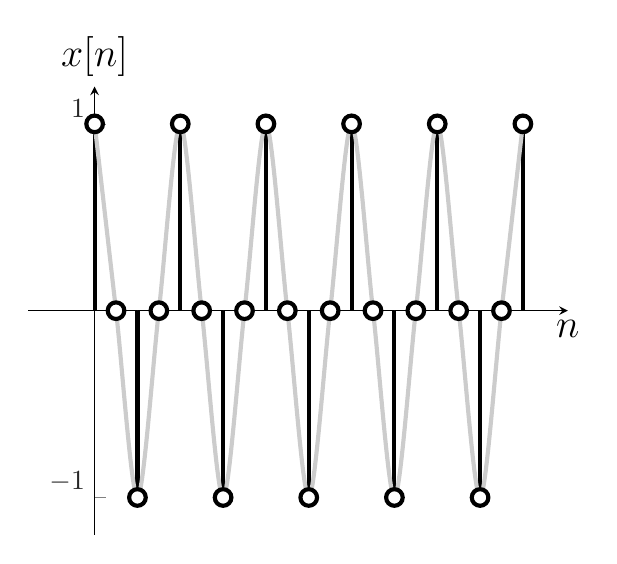
\begin{tikzpicture}
\begin{axis}[
axis lines*=middle,
enlargelimits = true,
ymin=-1,
ymax=1,
xmin=-1,
xmax=20,
axis line style={->,>=stealth},
xlabel={\Large $n$},
ylabel={\Large $x[n]$},
yticklabel style = {yshift=0.2cm},
xticklabel style = {yshift=-0.1cm},
every axis x label/.style={
	at={(ticklabel* cs:1)},
	anchor=north,
},
every axis y label/.style={
	at={(ticklabel* cs:1)},
	anchor=south,
},
ytick={-1, 1},
xtick=\empty,
every outer y axis line/.append style={white!15!black},
every y tick label/.append style={font=\color{white!15!black}},
legend style={draw=white!15!black,fill=white,legend cell align=left}]
\addplot [ycomb, mark=*, fill=white, mark options={scale=1.5, fill=white}, line width=1.5pt, forget plot]
table[row sep=crcr]{
	0 1 \\
	1 6.1232e-17 \\
	2 -1 \\
	3 -1.837e-16 \\
	4 1 \\
	5 3.0616e-16 \\
	6 -1 \\
	7 -4.2863e-16 \\
	8 1 \\
	9 5.5109e-16 \\
	10 -1 \\
	11 -2.4499e-15 \\
	12 1 \\
	13 -9.8034e-16 \\
	14 -1 \\
	15 -2.6948e-15 \\
	16 1 \\
	17 -7.3541e-16 \\
	18 -1 \\
	19 -2.9398e-15 \\
	20 1 \\
};

\addplot [smooth, black!20, line width=1.5pt, forget plot]
table[row sep=crcr]{
	0 1 \\
	1 6.1232e-17 \\
	2 -1 \\
	3 -1.837e-16 \\
	4 1 \\
	5 3.0616e-16 \\
	6 -1 \\
	7 -4.2863e-16 \\
	8 1 \\
	9 5.5109e-16 \\
	10 -1 \\
	11 -2.4499e-15 \\
	12 1 \\
	13 -9.8034e-16 \\
	14 -1 \\
	15 -2.6948e-15 \\
	16 1 \\
	17 -7.3541e-16 \\
	18 -1 \\
	19 -2.9398e-15 \\
	20 1 \\
};

\end{axis}
\end{tikzpicture}}};
	\node[below = 0.5mm of xc] {$x[n] = \cos(\omega_0n)$};	
	\node[below = 0.5mm of yc] {$y[n] = x[n]\ast h[n]$};
	}
	\onslide<4|handout:2>{
		\node[block, draw=none, scale=0.5] (rx_signal1) at ($(yc.north) + (1.5cm, 3cm)$) {\resizebox{12cm}{!}{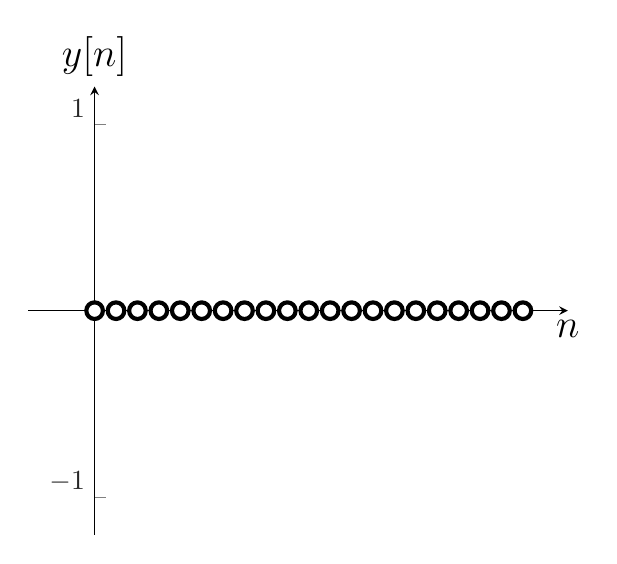
\begin{tikzpicture}
\begin{axis}[
axis lines*=middle,
enlargelimits = true,
ymin=-1,
ymax=1,
xmin=-1,
xmax=20,
axis line style={->,>=stealth},
xlabel={\Large $n$},
ylabel={\Large $y[n]$},
yticklabel style = {yshift=0.2cm},
xticklabel style = {yshift=-0.1cm},
every axis x label/.style={
	at={(ticklabel* cs:1)},
	anchor=north,
},
every axis y label/.style={
	at={(ticklabel* cs:1)},
	anchor=south,
},
ytick={-1, 1},
xtick=\empty,
every outer y axis line/.append style={white!15!black},
every y tick label/.append style={font=\color{white!15!black}},
legend style={draw=white!15!black,fill=white,legend cell align=left}]
\addplot [ycomb, mark=*, fill=white, mark options={scale=1.5, fill=white}, line width=1.5pt, forget plot, domain=0:20, samples=21] {0};

\end{axis}
\end{tikzpicture}}};
	}


\end{tikzpicture}}
\end{center}
\begin{align*}
h[n] = \frac{1}{4}(\delta[n] + \ldots + \delta[n-3]) \Longleftrightarrow H(z) = \frac{1}{4}(1 + z^{-1} + \ldots + z^{-3})
\end{align*}

\end{frame}

\begin{frame}
	
In Matlab \\
\texttt{> n = 0:20} \\
\texttt{> w0 = 0.2*pi} \\
\texttt{> x = cos(w0*n)} \\
\texttt{> y = filter([1 1 1 1]/4, 1, x)} \\
or equivalently \texttt{> y = conv([1 1 1 1]/4, x)} \\
\texttt{> stem(n, x)} \\
\texttt{> stem(n, y)} \\

\end{frame}


\end{document}
